\documentclass[smaller]{beamer}
\usepackage{beamerarticle}
\mode<presentation> {
  \usetheme[width=80pt]{Berkeley}
  \useinnertheme{circles}
  \usecolortheme{sidebartab}
  \setbeamercolor{structure}{fg=blue}
  % or ...

%  \setbeamercovered{transparent}
  % or whatever (possibly just delete it)
}

\usepackage[utf8]{inputenc}

\usepackage[english,russian]{babel}
\usepackage{listings}
\usepackage[pdftex,unicode]{hyperref}
%\usepackage[cp1251]{inputenc}
%\usepackage[utf8]{inputenc}
%\usepackage{listings}
%\usepackage[pdftex,unicode]{hyperref}
%\usepackage[english]{babel}
\usefonttheme{serif}
% Or whatever. Note that the encoding and the font should match. If T1
% does not look nice, try deleting the line with the fontenc.


\title{Fuzzy Patterns} % (optional, use only with long paper titles)

%\author % (optional, use only with lots of authors)
%{Вишневский В.В.\inst{1}}
\institute[Moscow State University] % (optional, but mostly needed)
{
  \inst{1}
  Moscow State University
}

\date[Patterns] % (optional, should be abbreviation of conference name)
{}
% - Either use conference name or its abbreviation.
% - Not really informative to the audience, more for people (including
%   yourself) who are reading the slides online

\AtBeginSubsection[] {
  \begin{frame}<beamer>
    \frametitle{Plan}
    \tableofcontents[currentsection,currentsubsection]
  \end{frame}
}
\begin{document}

\begin{frame}
  \titlepage
\end{frame}

\begin{frame}
  \frametitle{Plan}
  \tableofcontents
  % You might wish to add the option [pausesections]
\end{frame}



\section{Исследование поведения}


\begin{frame}	
  \frametitle{Задача исследования поведения}
Дана разметка поведения животного во времени.
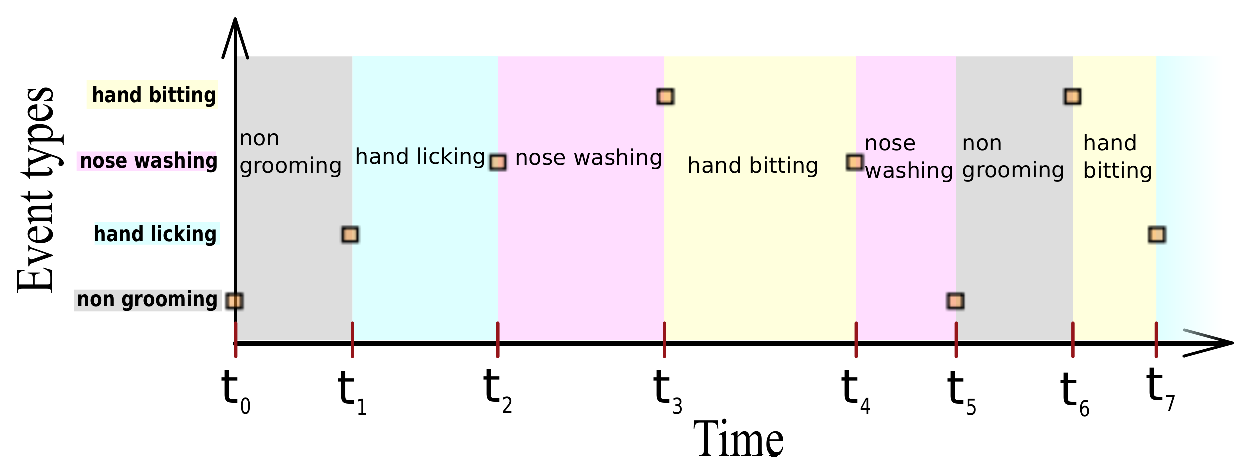
\includegraphics[scale=0.40]{beh_data.eps}
\end{frame}


\begin{frame}	
  \frametitle{Формальное описание данных}
\begin{itemize}
  \item Поведенческие события(акты): $A,B,C,D\dots$
  \item Каждый поведенческий акт происходит в некоторые моменты времени: $t_{A_1},\dots,t_{A_N}$. 
\end{itemize}
\begin{left}
\begin{tabular}[t]{p{12em}|p{12em}}
    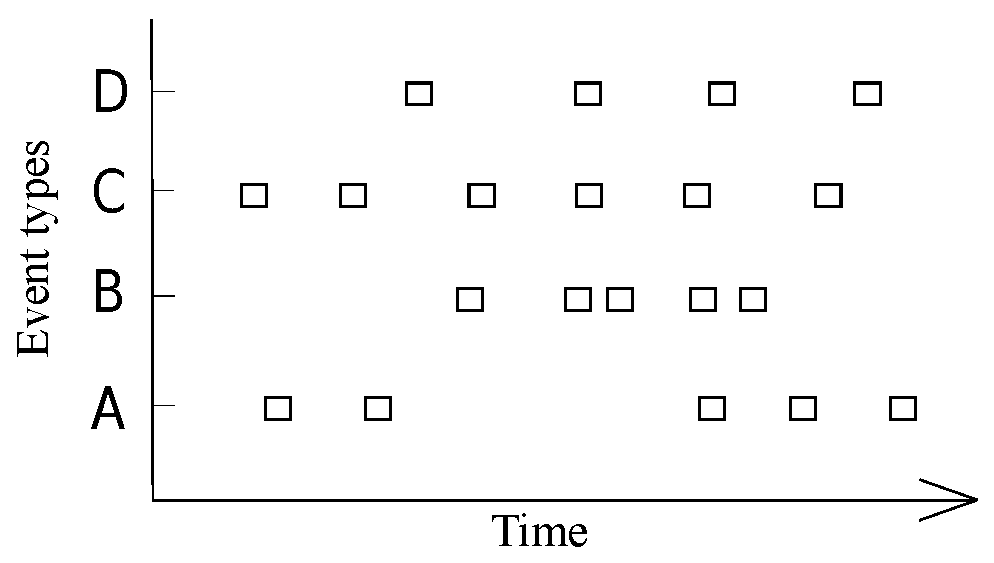
\includegraphics[scale=0.25]{NEWTS.eps} & 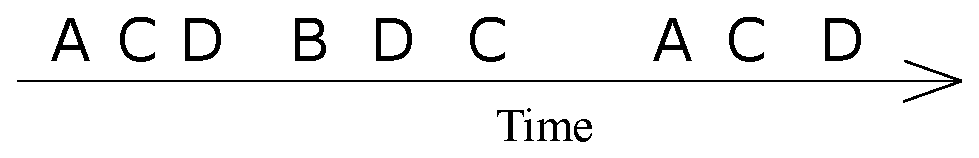
\includegraphics[scale=0.25]{TSNEW2.eps}\\
\end{tabular}
\end{left}
\end{frame}

\begin{frame}	
  \frametitle{Так выглядят реальные данные}
    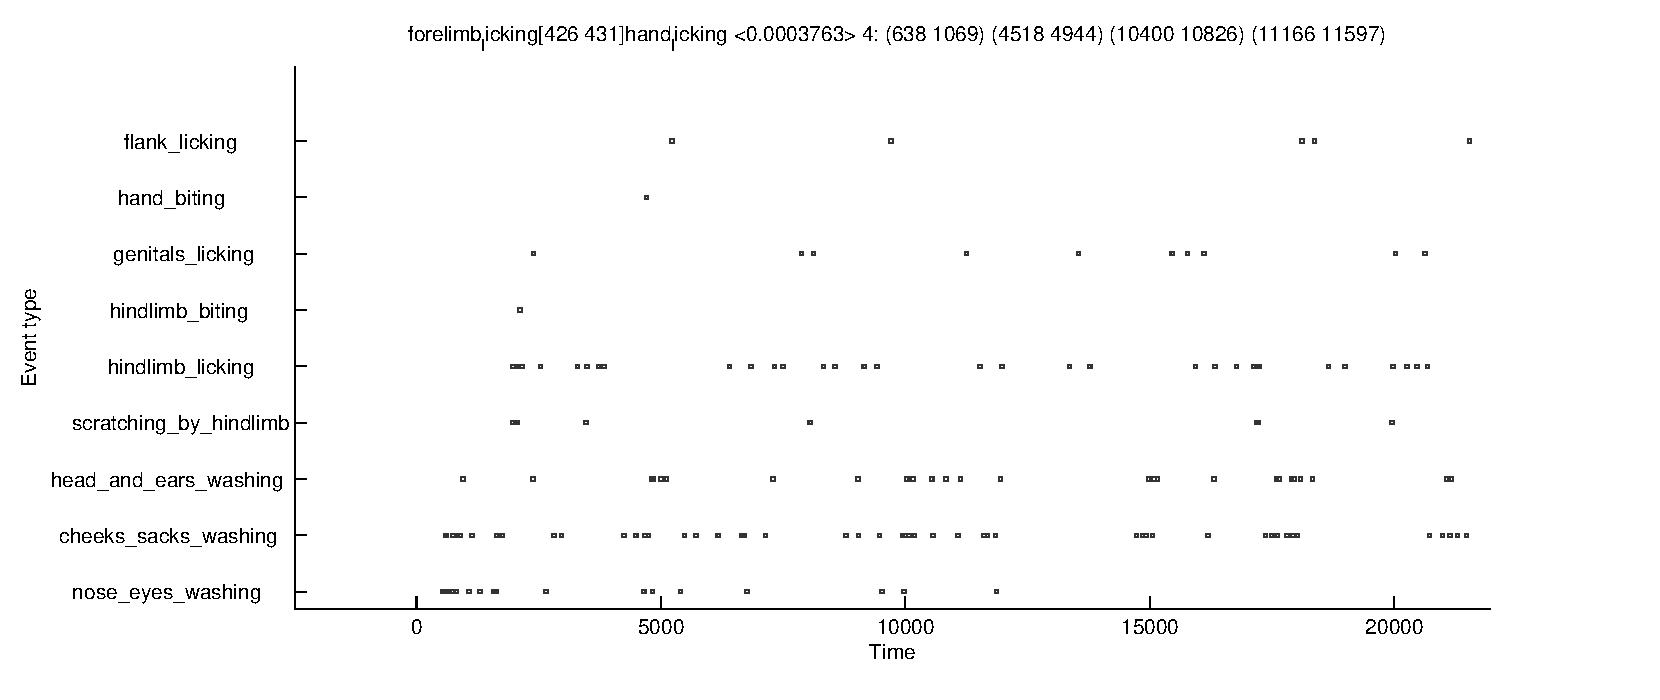
\includegraphics[scale=0.4]{TS.eps} 
\end{left}
\end{frame}

\begin{frame}	
  \frametitle{Что такое паттерн}
Паттерн~--- это последовательность событий(поведенческих актов), повторяющихся один за другим 
достаточно часто.
\end{frame}

\begin{frame}	
  \frametitle{Подход к поиску паттернов}
  Инициализируем множество паттернов псевдопаттернами(поведенческие акты). Потом итеративно повторяем:
  \begin{itemize}
   \item {\bf Конструирование:}Для всех пар паттернов проверить, повторяется ли один за другим достаточно часто. Если да, 
	то получаем новый паттерн. 
   \item {\bf Зачистка:} Удалить одинаковые паттерны, которые были сконструированы по-разному.
  \end{itemize}
\end{frame}

\begin{frame}	
  \frametitle{Общие замечания}
  \begin{itemize}
   \item Важно формально определить, что такое паттерн.
   \item Этапы конструирования и зачистки определяются заданием паттерна.
   \item Как проверить, повторяется ли один паттерн за другим достаточно часто?
  \end{itemize}
\end{frame}

\subsection{Т-Паттерны}
\begin{frame}	
  \frametitle{Понятие Т-Паттерна(M.S. Magnusson)}
  \begin{itemize}
   \item События соединеятся критическими интервалами. $A[dA_l,dA_r]B[dB_l,dB_r]C\dots F$. 
   \item Критический интервал ($A[d_1,d_2]B$) -- это связь между двумя паттернами, означающая, что второй паттерн($B$) промежутке $[d_1,d_2]$ 
после появления первого паттерна($A$) чаще, чем ожидается.
\\ 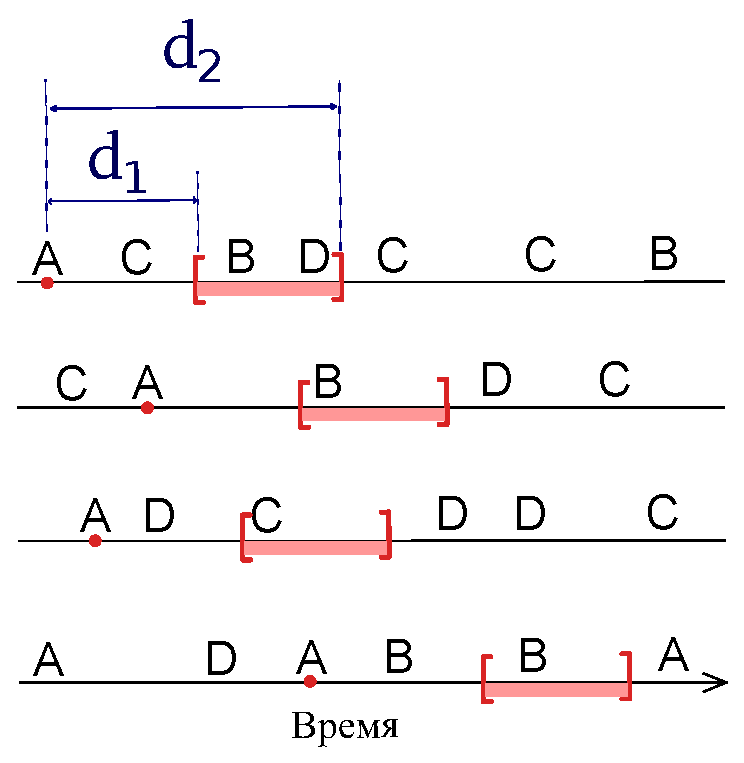
\includegraphics[scale=0.30]{TPTSn.eps} 
  \end{itemize}
\end{frame}

\subsubsection{Этап конструирования}
\begin{frame}	
  \frametitle{Этап конструирования}
    Существуют ли такие $d_1$ и $d_2$, что $A[d_1,d_2]B$ является критической связью?
\begin{itemize}
   \item Перебираем все возможные пары $d_1$ и $d_2$.
   \item Проверяем, значимость связи $[d_1, d_2]$. <<Чаще чем ожидается>>.
  \end{itemize}
  Ожидается что паттернов нету. Значит времена появления событий распределены равномерно.
\end{frame}

\begin{frame}	
  \frametitle{Статистический критерий}
\begin{itemize}
 \item $N_A, N_B$~--- количество появлений событий $A$ и $B$.

  \item $N_t$~--- продолжительность времени наблюдения.

  \item $d=d_2-d_1+1$~--- ширина тестируемого интервала.

  \item $P(A)=\frac{N_A}{N_t}$~--- вероятность наблюдать событие $A$ в какой-либо момент времени. 
  
  \item $P(\neg A) = 1 - P(A)$ 
  
  \item $1-P(\neg A)^d$~-- вероятность наблюдать событие $A$ в каком-либо интервале длины d.

  \item $N_{AB}$~--- Количество интервалов $A[d_1, d_2]$, в которых есть событие $B$.

  \item $\rho = P(\geqslant N_{AB}) = 1 - \sum_{i=0}^{N_{AB}-1}C_{N_{A}}^i( 1-P(\neg B)^d )^iP(\neg B)^{d(N_{A}-i)}$
\end{itemize}
\end{frame}

\begin{frame}	
  \frametitle{Статистический критерий}
\begin{itemize}
 \item Итак, мы имеем $\rho=\rho(N_A,N_B,N_t,N_{AB},d)$~---вероятность текущей конфигурации
событий, предполагая равномерное распределение данных(паттернов нету).
  \item Если $\rho<\alpha\approx0.05$, то считаем что существует критическая связь $A[d_1,d_2]B$.
  \item Обычно требуется $N_{AB}>N_{min}\approx3$.
  \item Можно ставить разные уровни значимости для паттернов разной длины.
  \item Для двух паттернов $A$ и $B$ могут существовать разные критические интервалы $[d_1, d_2]$.
      Какой выбирать?
\end{itemize}
\end{frame}

\subsubsection{Этап зачистки}
\begin{frame}	
  \frametitle{Типы <<лишних>> паттернов}
\begin{itemize}
 \item {\bf Дубликаты:} $(AB)(CD)$ и $(A(BC))D$
  \\ 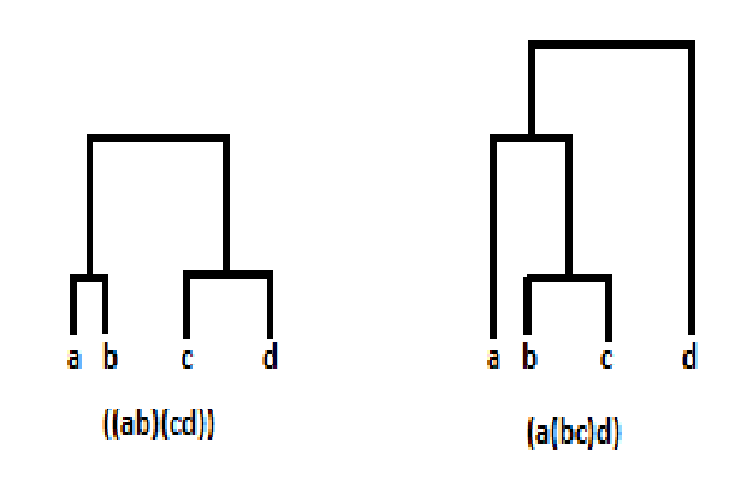
\includegraphics[scale=0.37]{dup_tree.eps} 
 \item {\bf Неполные копии:} $(BCD)$ не встречается вне $(ABCD)$
  \\ 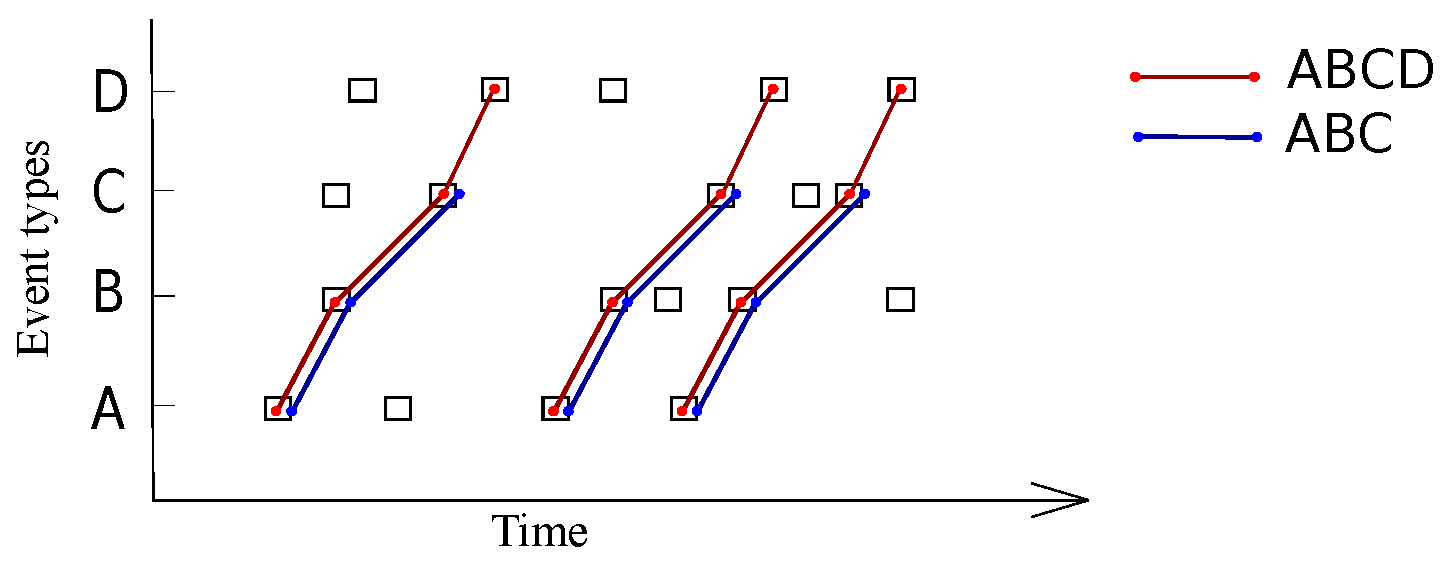
\includegraphics[scale=0.30]{dup_2.eps} 
\end{itemize}
\end{frame}

\subsubsection{Заключение}
\begin{frame}	
  \frametitle{Правило удаления}
 Паттерн $A$ считается менее полным, чем паттерн $B$, если $A$ и $B$ появляются одинаково часто и все события,
 возникающие в $A$ также возникают в $B$.
\end{frame}


\begin{frame}	
  \frametitle{Параметры метода}
 \begin{tabular}{ |p{5em} | p{4em} | p{4em} | p{8em}| }
    
    \hline
    \bf{Параметр} & \bf{ Область значений} & \bf{ Значение по умолчанию} & \bf{ Смысл } \\
    \hline
    $\alpha$ & $[0,1]$ & 0.995 & Уровень значимости паттернов \\ \hline
    $N_{min}$ & $[0, +\infty]$ & 3 & Минимальное число появлений паттерна  \\ \hline
  \end{tabular}
  \begin{itemize}
    \item Задание стратегии поиска критических интервалов.
    \item Дополнительные ограничения.
  \end{itemize}
\end{frame}

\begin{frame}	
  \frametitle{Параметры метода}
 \begin{itemize}
    \item Удовлетворительно работает на поведенческих данных.
    \\ 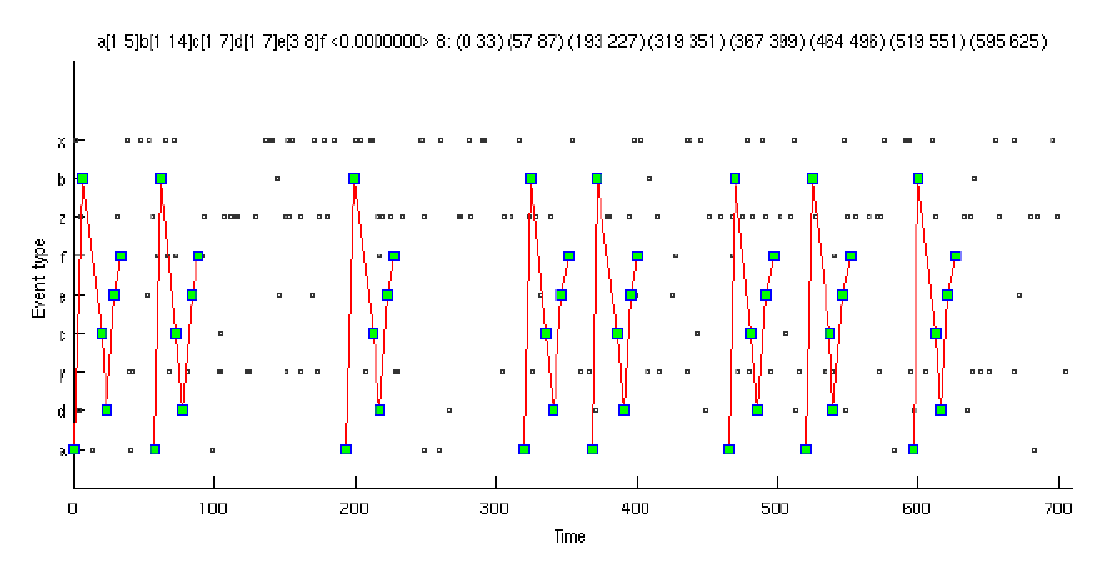
\includegraphics[scale=0.50]{resultex.eps} 
    \item Алгоритм очень чувствителен к пропускам в данных.
  \end{itemize}
\end{frame}

\subsection{Fuzzy Patterns}
\begin{frame}
  \frametitle{Предпосылки}
  \begin{itemize}
  \item Еще раз: Т-Паттерны очень чувствительны к пропускам в данных,
  \item новый тип паттернов, 
  \item схожий с Т-Паттернами метод поиска,
  \item правдоподобие паттерна в каждой точке.
   \end{itemize}
\end{frame}

\subsubsection{Правдоподобие паттерна}
\begin{frame}
\frametitle{Представление паттерна}
 \begin{itemize}
  \item Паттерн состоит из элементарных событий,
  \item каждое событие паттерна характеризуется смещением и разбросом от предыдущего события(гармошка),
  \item либо от предыдущего мат. ожидания(занавеска),
  \item $P=A[\mu_A,\sigma_A]B[\mu_B,\sigma_B]C[\mu_C,\sigma_C]$
 \end{itemize}
\begin{left}
\begin{tabular}[t]{p{12em}|p{12em}}
    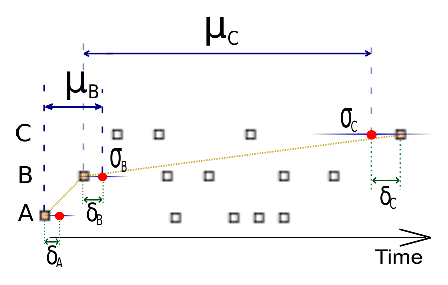
\includegraphics[scale=0.6]{il1.eps} & 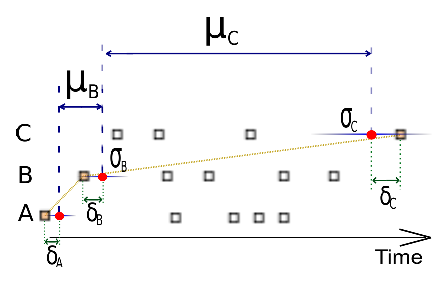
\includegraphics[scale=0.6]{il2.eps}\\
\end{tabular}
\end{left}
\end{frame}  


\begin{frame}
  \frametitle{Функция потерь}
  \begin{itemize}
  \item Штраф за пропуск $x$ событий в паттерне длины $N$:
  $$
  f_{LOSS}(x,N)= \begin{cases}
   \exp\bigl(-\frac{\lambda x}{N}\bigr), & x < N, \\
   0,                                    & x=N.
   \end{cases}
  $$
  \item $\lambda$ определяет уровень нечеткости паттернов.
   \end{itemize}
   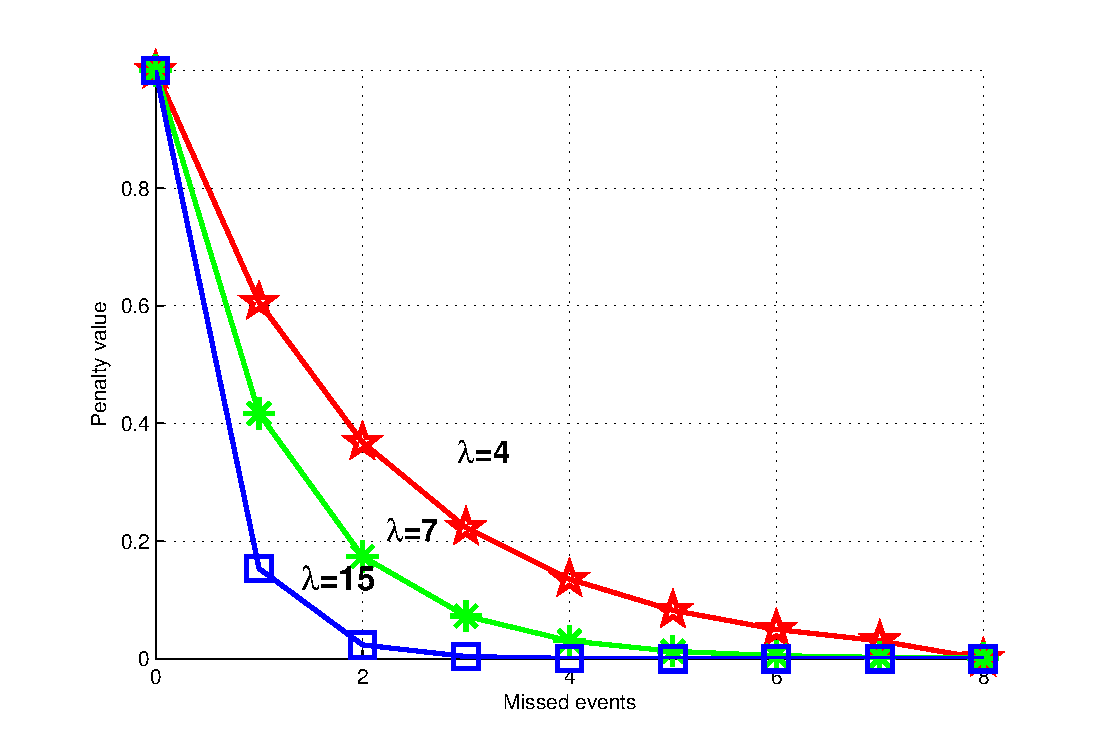
\includegraphics[scale=0.35]{MB_LF.eps}
\end{frame}

\begin{frame}
  \frametitle{Правдоподобие}
   $$L_P(\varepsilon)=f_{LOSS}(N_-,N)\prod_{i=1}^{N}\biggl( \frac1{\sqrt{2\pi}\sigma_i }\biggr)  \prod_{i=1}^{N_+}\exp\biggl(- \frac{\delta_i^2}{2\sigma_i^2}\biggr) $$
   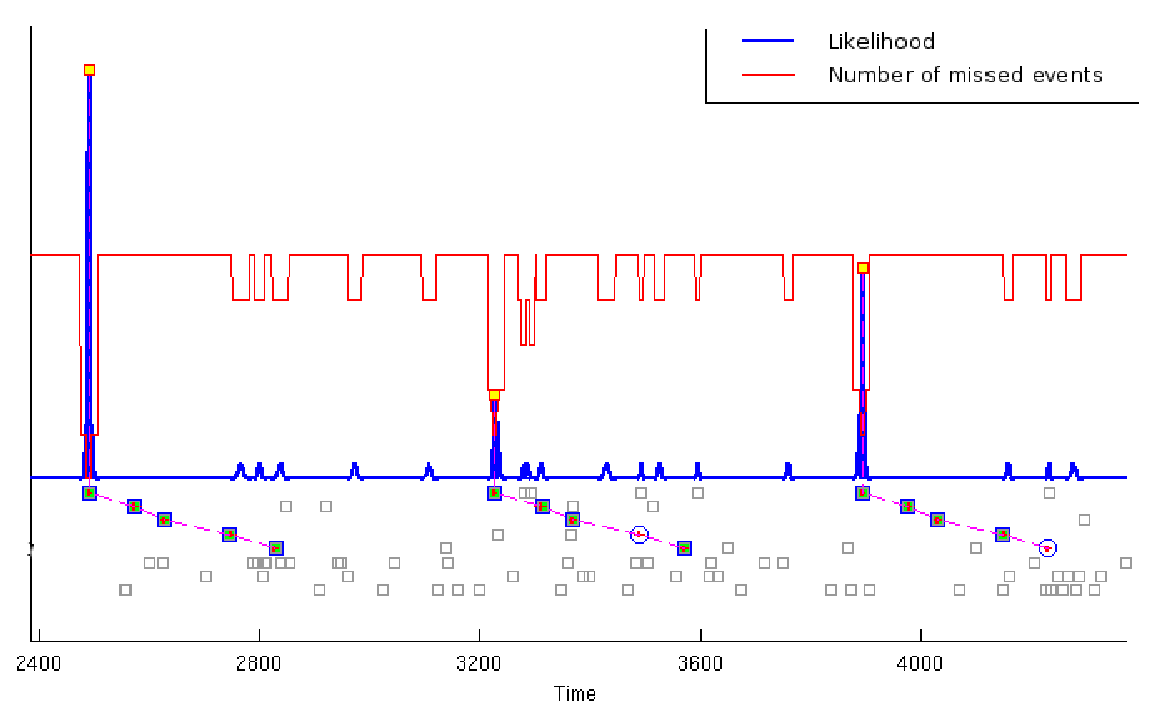
\includegraphics[scale=0.4]{norm_12_of_14.eps}
\end{frame}

\begin{frame}
  \frametitle{Правдоподобие}
   Правдоподобие можно считать с конца, или начиная с $i$-го события.
    $$L_{P,m}=L_P(\varepsilon+\sum_{j=1}^m\mu_j)$$
   \begin{center}
   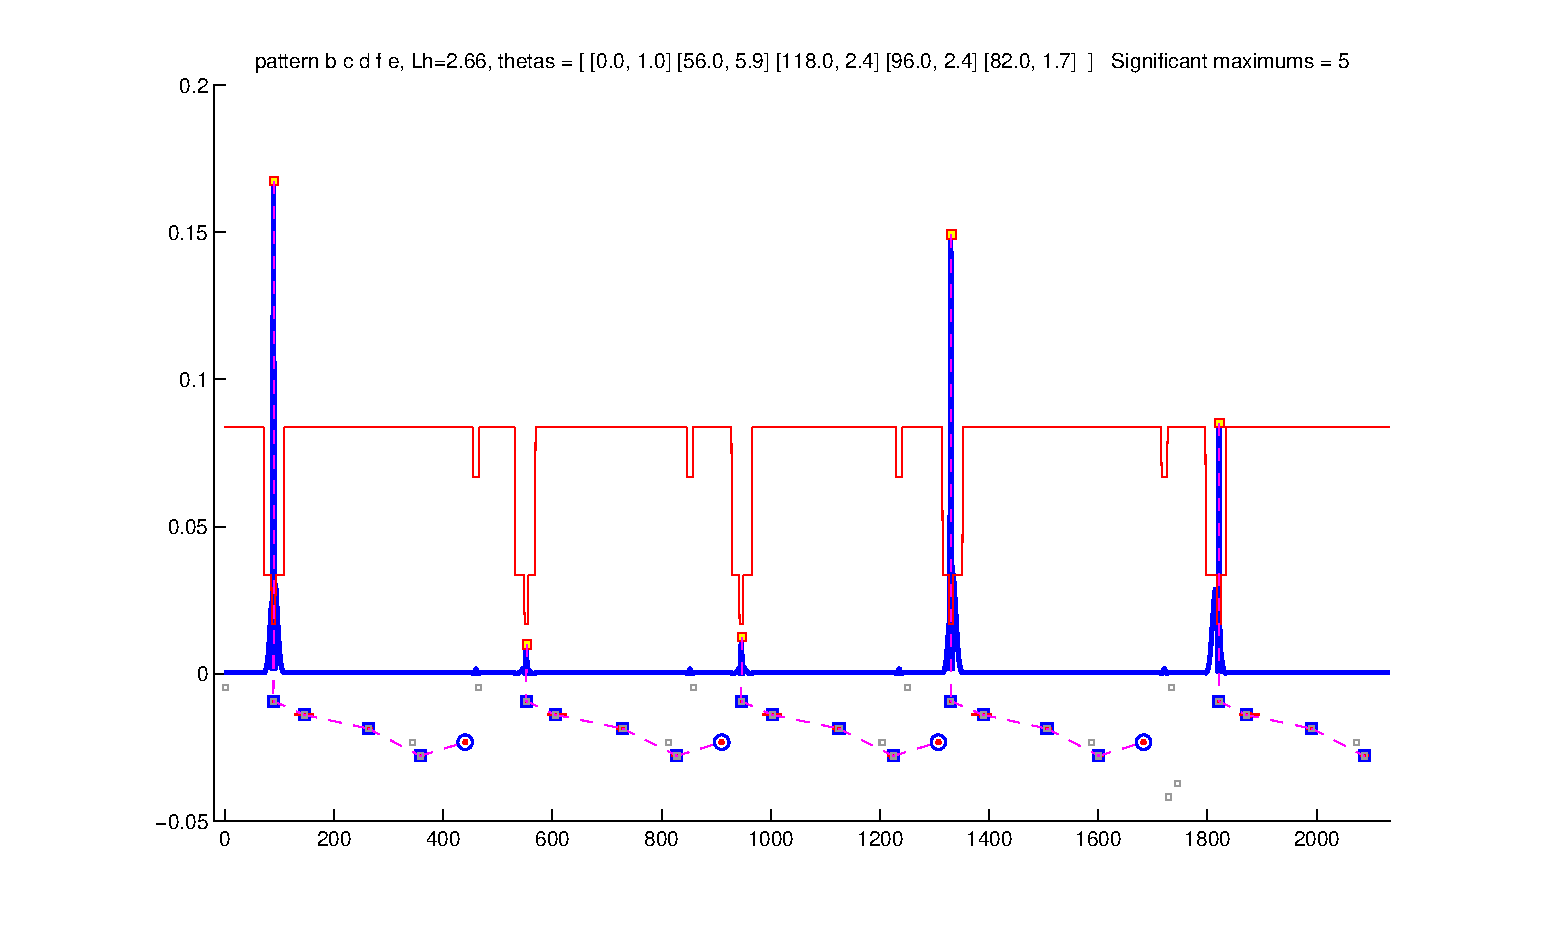
\includegraphics[scale=0.2]{pat1.eps}
   \\
   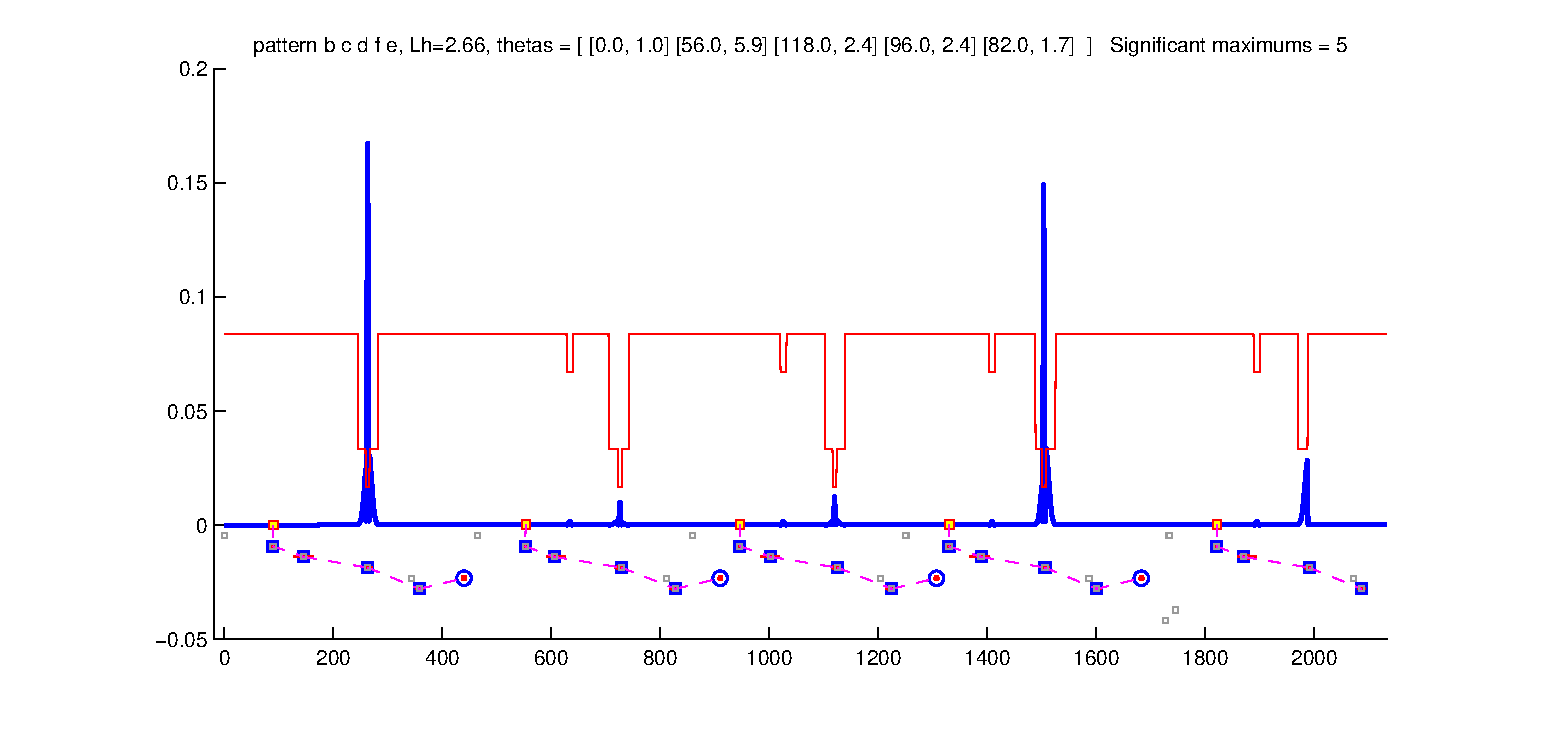
\includegraphics[scale=0.2]{pat2.eps}
   \end{center}
\end{frame}

\subsubsection{Этап конструирования}
\begin{frame}
  \frametitle{Межточечное распределение}
  \begin{itemize}
   \item Рассматриваем распределение расстояний между концом левого и началом правого паттерна,
   \item отсечение окном ширины $M$,
   \item вводим $g_{\mu,\sigma}(\rho_l)=\exp\bigl(-\frac{(\rho_l-\mu)^2}{2\sigma^2}\bigr)$~-- это статистическая модель связи между событиями,
   \item подсчитываем $k=\sum_{l=1}^Q w_lg_{\mu,\sigma}(\rho_l).$
   \end{itemize}
   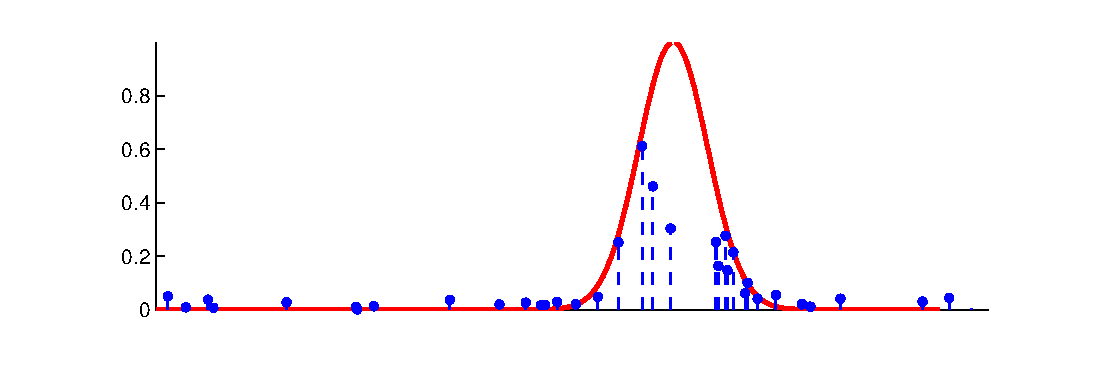
\includegraphics[scale=0.4]{weights.eps}
\end{frame}

\begin{frame}
  \frametitle{Гипотеза о случайности распределения}
  \begin{itemize}
    \item Если в данных нету закономерностей:
    \begin{itemize}
        \item  с.в. $w$ и $\rho_l$~-- независимы,
        \item  $\rho_l \in U[0,M]$,
        \item $Y=\sum_{l=1}^Qw_lg_{\mu,\sigma}(\rho_l)$, 
    \end{itemize}
    \item Используя Ц.П.Т, можно показать, что:
    $$Y\sim \mathcal{N}\biggl( \frac{\sum_{i=1}^Q w_i}MS, \frac1{M^2}\biggl[ MS\sqrt{2}\sum_{i=1}^Q w_i^2-\frac{(\sum_{i=1}^Q w_i)^2}QS^2 \biggr] \biggr)$$
    \item ищем $\mu$ и $\sigma$:
    $$\frac{k-\mathbb{E}Y}{\sqrt{\mathbb{D}Y}}\to\min_{\mu,\sigma},$$
    \item сравниваем с квантилью нормальмального распределения; $\omega$.
   \end{itemize}
\end{frame}

\subsubsection{Этап зачистки}
\begin{frame}
  \frametitle{Виды <<лишних>> паттернов}
  \begin{itemize}
   \item {\bf Дубли:} (AB)(CD), (ABC)D,
   \item {\bf Неполные копии:} (BCD) не встречается вне (ABCD).
   \item похожесть паттернов по вектору правдоподобия $\overrightarrow{L}$, коэффициент корреляции:
   $$cor(\overrightarrow{L_1}, \overrightarrow{L_2}) = \frac{\overrightarrow{L_1}\overrightarrow{L_2}^T}{\sqrt{\overrightarrow{L_1}\overrightarrow{L_1}^T}\sqrt{\overrightarrow{L_2}\overrightarrow{L_2}^T}}$$
   \end{itemize}
\end{frame}

\begin{frame}
  \frametitle{Процедура удаления}
  
  Есть паттерн $P_1$ и $P_2$.
  Если все события, которые входят в $P_1$ так же 
  входят в $P_2$ и  $\exists m: cor(\overrightarrow{L_{P_1,m}}, \overrightarrow{L_{P_2,1}}) > \nu$, то  
  $P_1$ удаляется.
  
\end{frame}

\subsubsection{Заключение}
\begin{frame}
  \frametitle{ Parameters of algorithm }
    
    \begin{tabular}{ |p{5em} | p{4em} | p{4em} | p{8em}| }
    
    \hline
    \bf{Parameter} & \bf{ Possible values} & \bf{ Default value} & \bf{ Has influence on } \\
    \hline
    \omega & $[0,1]$ & 0.995 & Significance of pattern \\ \hline
    \mu & $[0, +\infty]$ & 3 & Minimal pattern occurrences  \\ \hline \hline
	\lambda & $[0, +\infty]$ & 6 & Fuzziness of patterns  \\  \hline    
    \nu & $[0,1]$ & 0.7 & Similarity of patterns for elimination \\ \hline
    $M$ & $[0,N_t]$ & None & Max time span between events in patterns \\ \hline
    \end{tabular}

\end{frame}

\begin{frame}
  \frametitle{ Пример }
       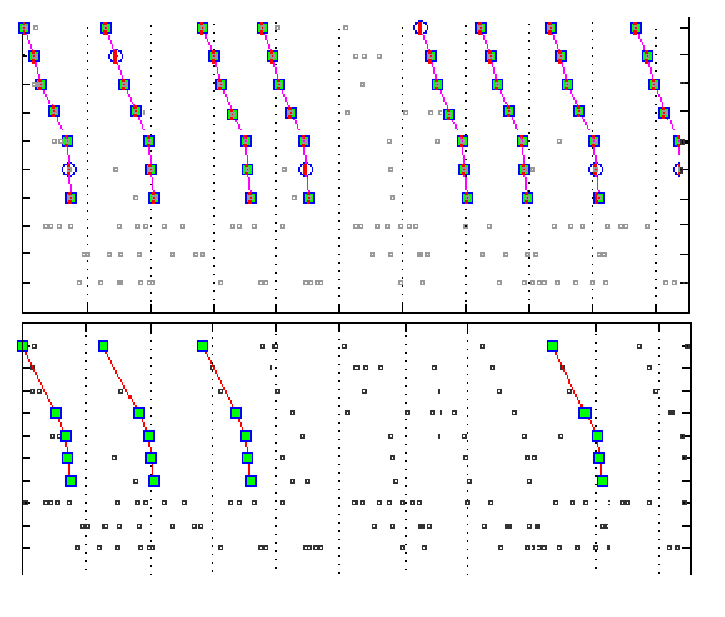
\includegraphics[scale=0.6]{comp.eps} 
\end{frame}

\section{Задача определения концентрации ферментов}
\subsection{Калибровка}
\begin{frame}
  \frametitle{Химическая кинетика}
  Есть субстрат $S$, преобразуемый ферментом $E$ в конечный продукт реакции $P$.
  $$ E+S\rightarrow E+P$$
  Уравнение Михаэлиса~--~Ментен:
  $$
    \begin{align}
     & v=\frac{dP(t)}{dt}=\frac{V_{max}S(t)}{K_M+S(t)}\\
     & V_{max}=k_{cat}E \\
     & S(0)=S_0, P(0)=0 \\
     & S(t)+P(t)=S_0 
     \end{align}
  $$
\end{frame}

\begin{frame}
  \frametitle{Исходные данные}
  После интегрирования, учитывая начальные условия:
  $$P(t)=k_{cat}Et+K_{M}\ln\biggl( 1-\frac{P(t)}{S_0}\biggr)$$
  \\ 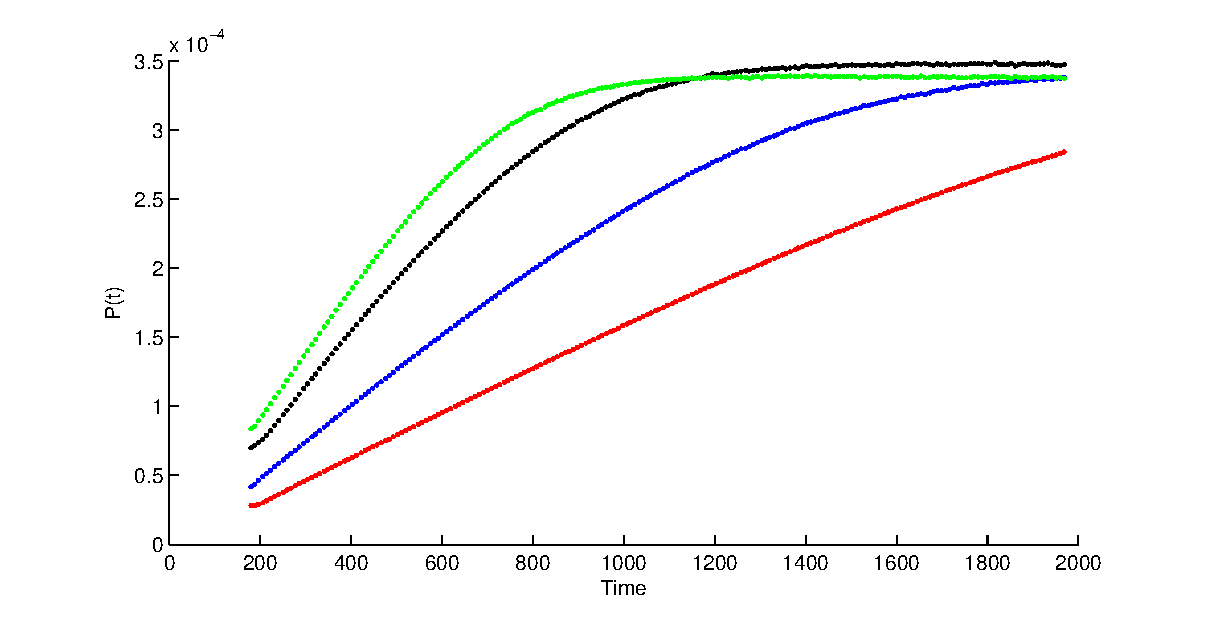
\includegraphics[scale=0.5]{Pt_raw.eps}
\end{frame}

\begin{frame}
  \frametitle{Формулировка задания}
    \begin{itemize}
   \item Данные о реакции одного фермента и одного субстрата.
   \item Даны измерения $P(t)$.
   \item 8 разных концентраций фермента($E$). По 5 экспериментов с каждыми значением концентрации $E$.
   \item $S_0$ должно быть одинаково во всех экспериментах.
   \item Найти значения констант $V_{max}$ и $K_M$ для данной пары фермент~--~субстрат.
   \end{itemize}
\end{frame}

\begin{frame}
  \frametitle{Сглаживание}
   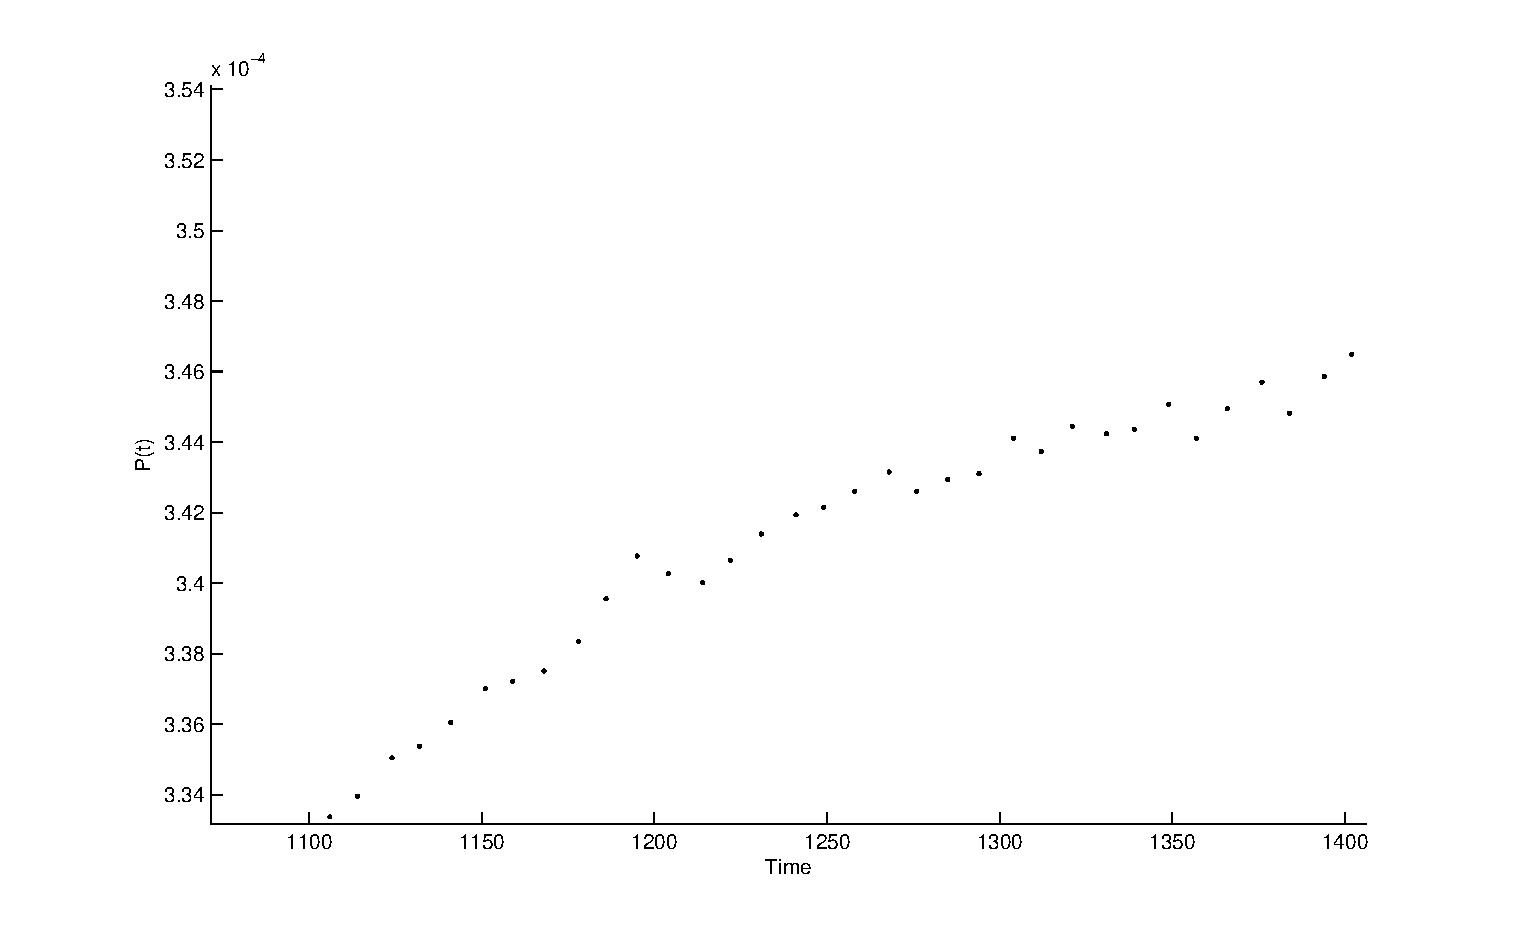
\includegraphics[scale=0.5]{Pt_fuzzy.eps}
\end{frame}

\subsection{Сглаживание}
\begin{frame}
  \frametitle{Как восстанавливать функцию}
    \begin{itemize}
   \item На отрезке $[a,b]$ даны значения целевой функции $f(x_i)=y_i, i=1,\dots,l$.
   \item Требуется восстановить целевую функцию $\hat{f}(x), x\in[a,b]$.
   \item Интерполирование. Найти $\hat{f}:[a,b]\rightarrow\mathbb{R}$ такую, что $y_i=\hat{f}(x_i), i=1,\dots,l$
   \item Регрессия. Curve fitting. Найти $\hat{f}:[a,b]\rightarrow\mathbb{R}$, минимизирующую ошибку $\sum_{i=1}^l \bigl(\hat{f}(x_i)-y_i\bigr)^2$.\\
	  Точнее $y_i=\hat{f}(x_i)+\varepsilon_i$
   \end{itemize}
\end{frame}

\begin{frame}
  \frametitle{Методы}
    \begin{itemize}
   \item Kernel smoothing
   \item Линейная регрессия. Polynomial fitting.
   \item Локальная регрессия.
   \item Сплайны.
   \end{itemize}
\end{frame}

\begin{frame}
  \frametitle{Kernel smoothing}
   \begin{itemize}
    \item $\hat{f}(x) = \frac{  \sum_{i=1}^l\biggl[ W\bigl( \frac{x_i-x}h \bigr)y_i \biggr] }{ \sum_{i=1}^lW\bigl( \frac{x_i-x}h \bigr) }$
    \item $W(h)$~--- весовая функция. Например, $W(u)=exp(-u^2)$.
    \item Проблема выбора ширины окна.
    \item Краевые эффекты.
   \end{itemize} 
\end{frame}

\begin{frame}
  \frametitle{Kernel smoothing}
   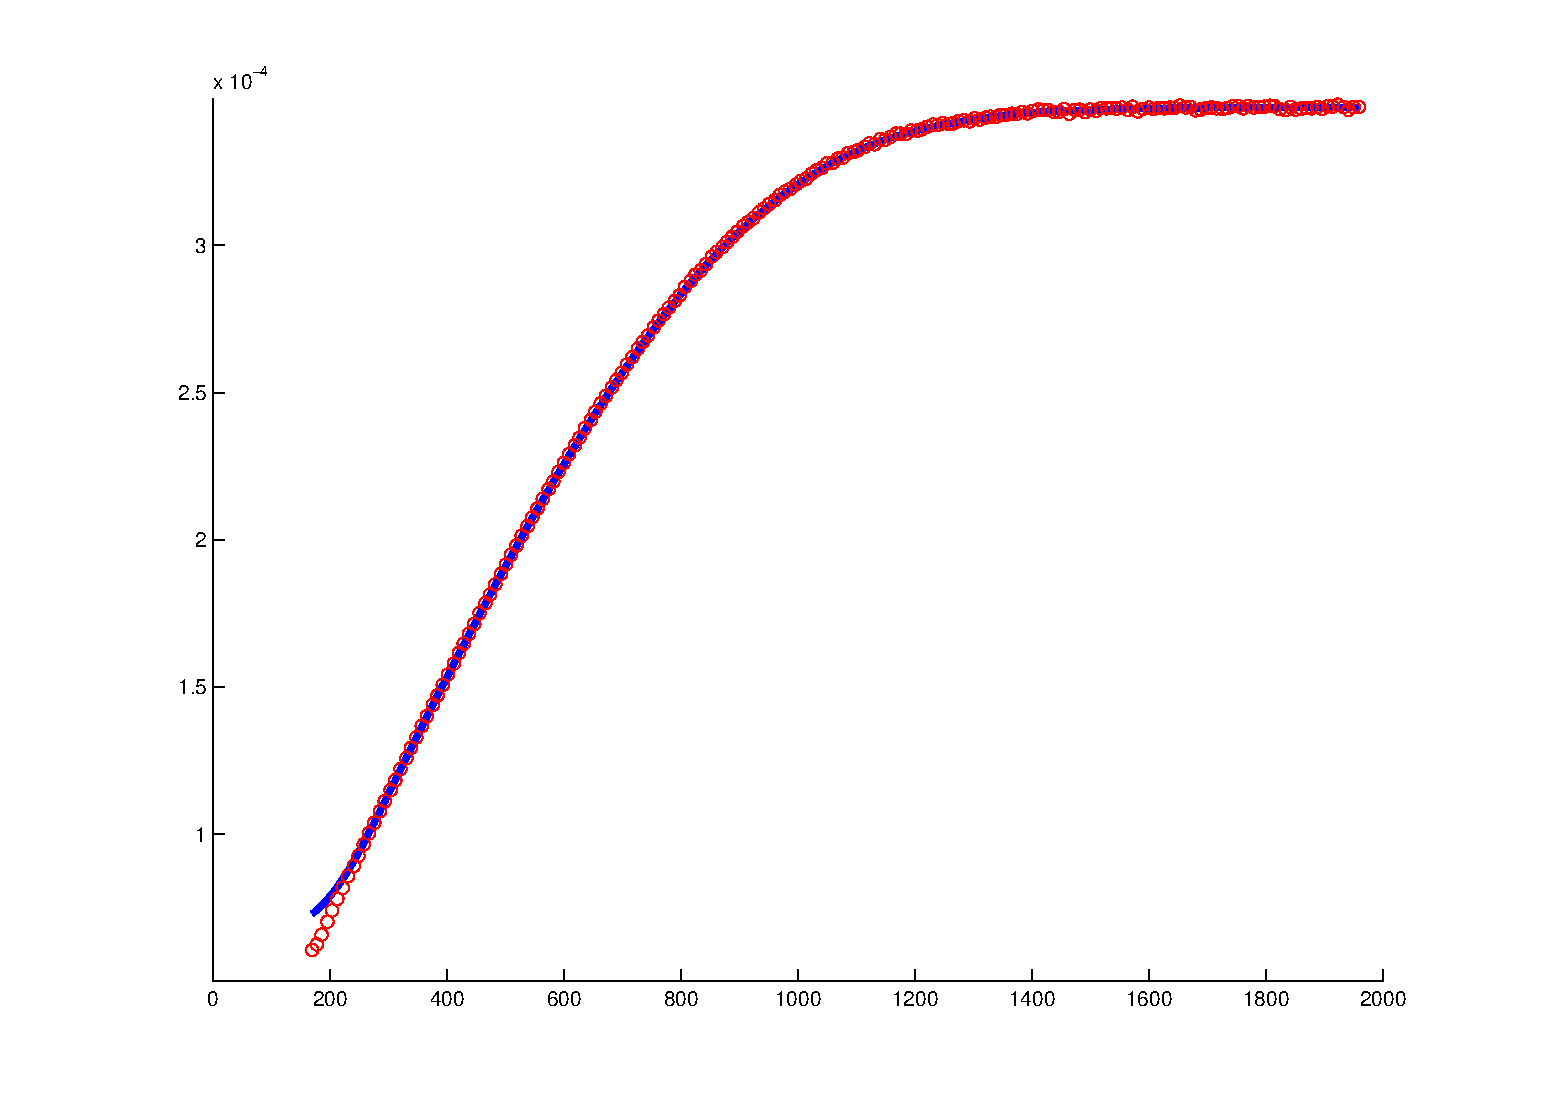
\includegraphics[scale=0.4]{kern_smooth.eps} 
   
\end{frame}

\begin{frame}
  \frametitle{Kernel smoothing}
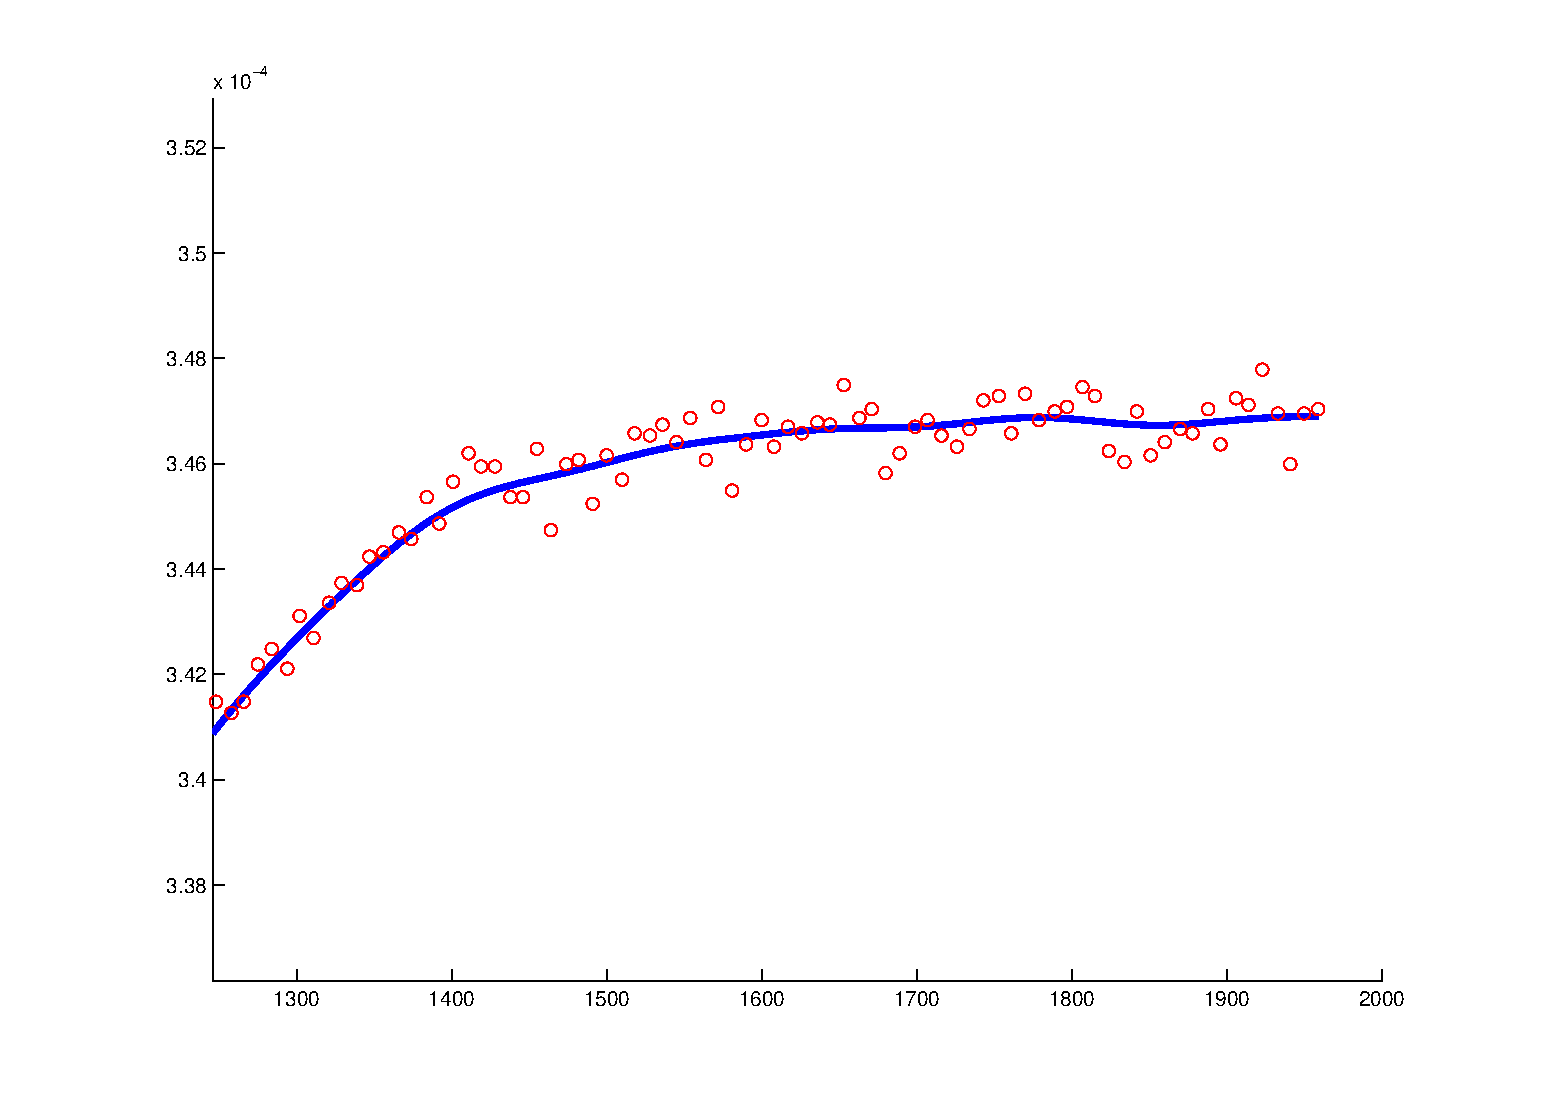
\includegraphics[scale=0.4]{kern_smooth_b.eps}
\end{frame}

\begin{frame}
  \frametitle{Линейная регрессия. Polynomial fitting}
   \begin{itemize}
    \item Предполагаем, что $\hat{f}(x) = w_mx^m+w_{m-1}x^{m-1}+...+w_1x+w_0$.
    \item Настраиваем веса $w_i, i=1,\dots,m$ методом наименьших квадратов. 
    \item Проблема выбора степени полинома.
   \end{itemize}
\end{frame}

\begin{frame}
  \frametitle{Линейная регрессия. Polynomial fitting}
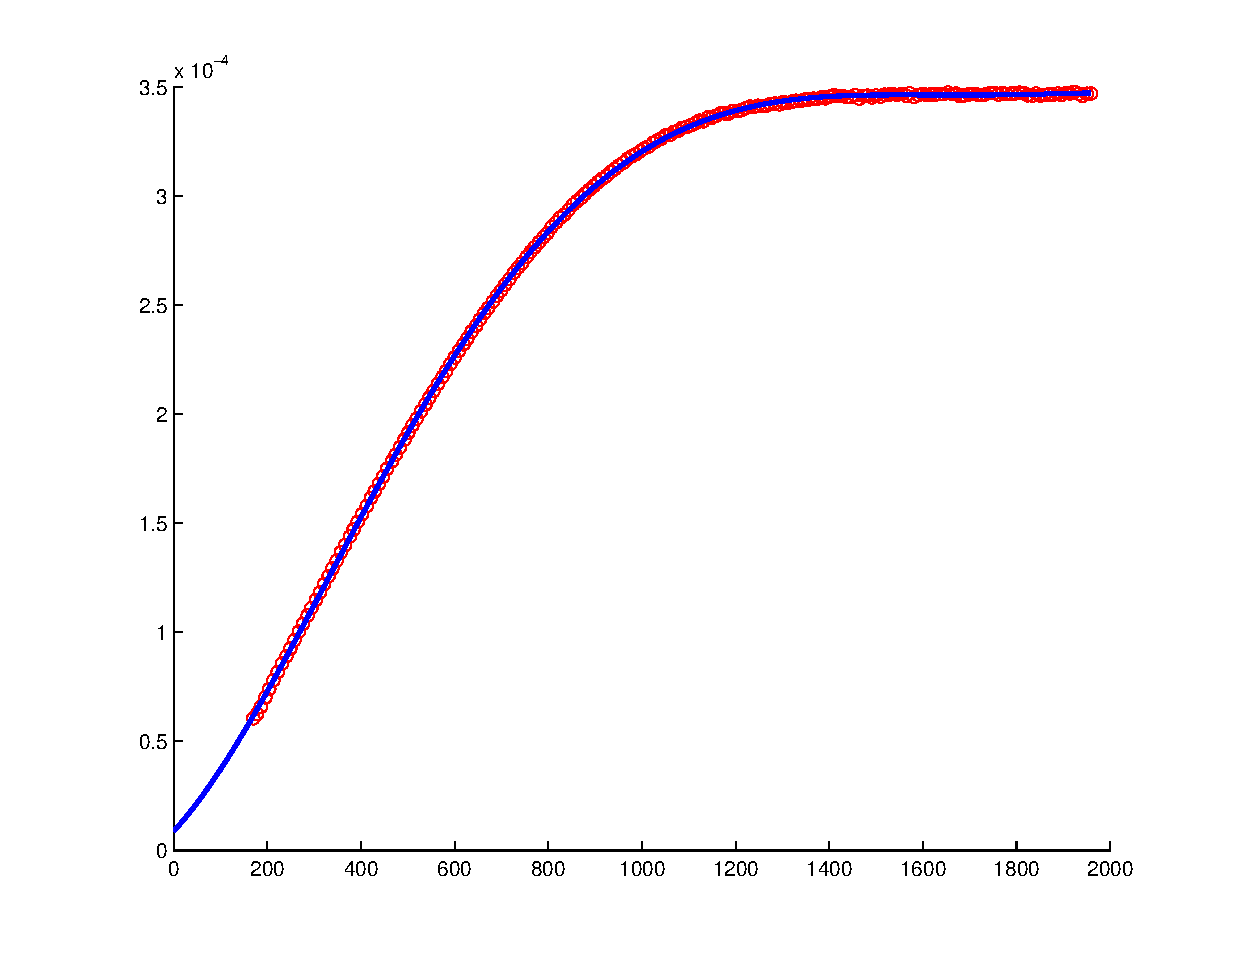
\includegraphics[scale=0.4]{poly_fit.eps}
\end{frame}

\begin{frame}
  \frametitle{Линейная регрессия. Polynomial fitting}
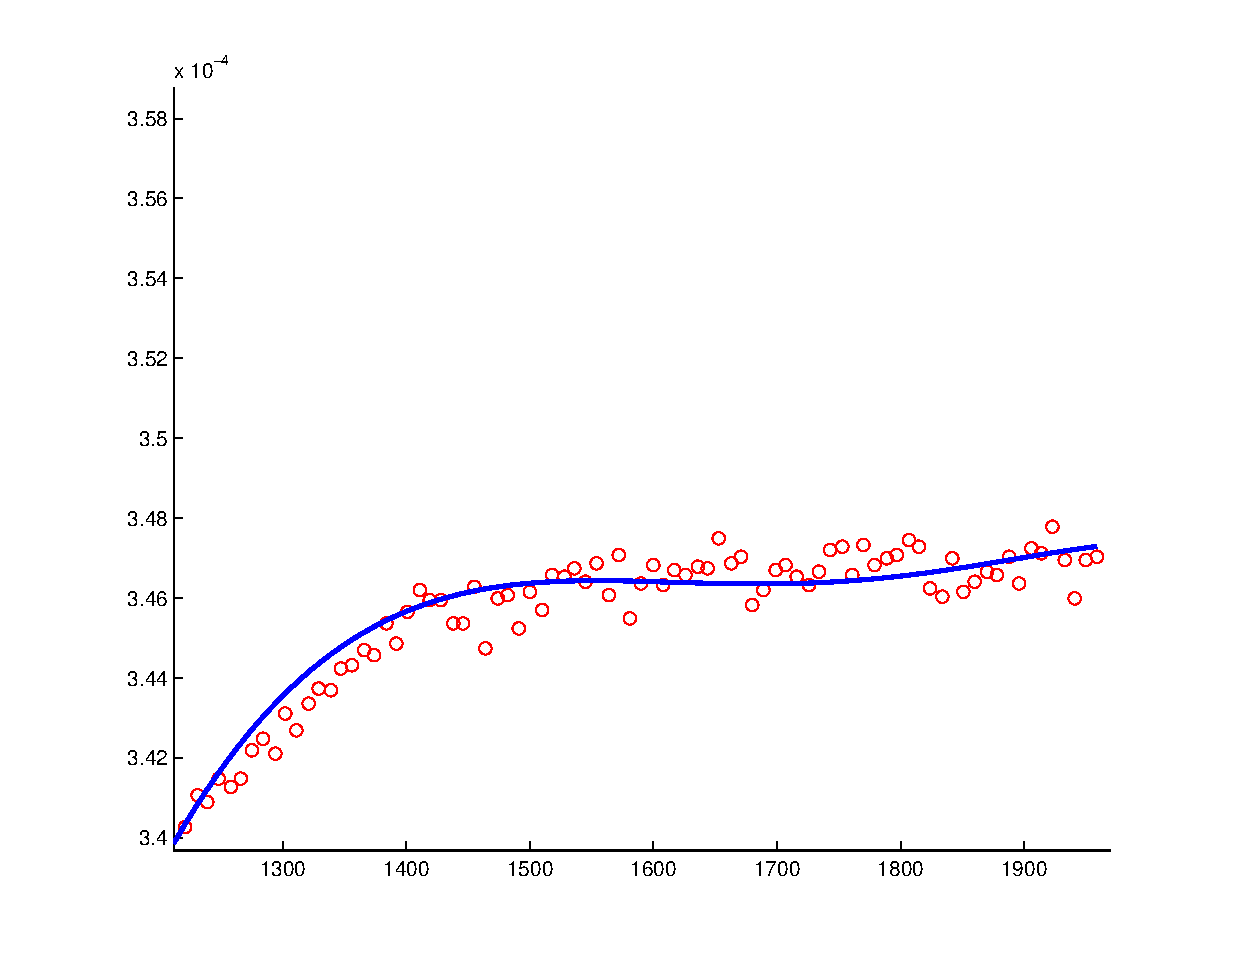
\includegraphics[scale=0.4]{poly_fit_b.eps}
\end{frame}


\begin{frame}
  \frametitle{Локальная регрессия}
   \begin{itemize}
    \item Восстанавливается линейная регрессия в окрестности каждой точки. 
    \item $\hat{f}(x) \approx a_0(x)+a_1(x)x$
    \item В каждой точке $a_0$ и $a_1$ могут быть найдены, решая следующую задачу взвешенных наименьших квадратов:
      $$ argmin_{a_0, a_1} \sum_{i=1}^l W \biggl( \frac{x_i-x}h \biggr) \bigl[y_i-a_0 +a_1x\bigr]^2 $$
   \end{itemize}
\end{frame}

\begin{frame}
  \frametitle{Локальная регрессия}
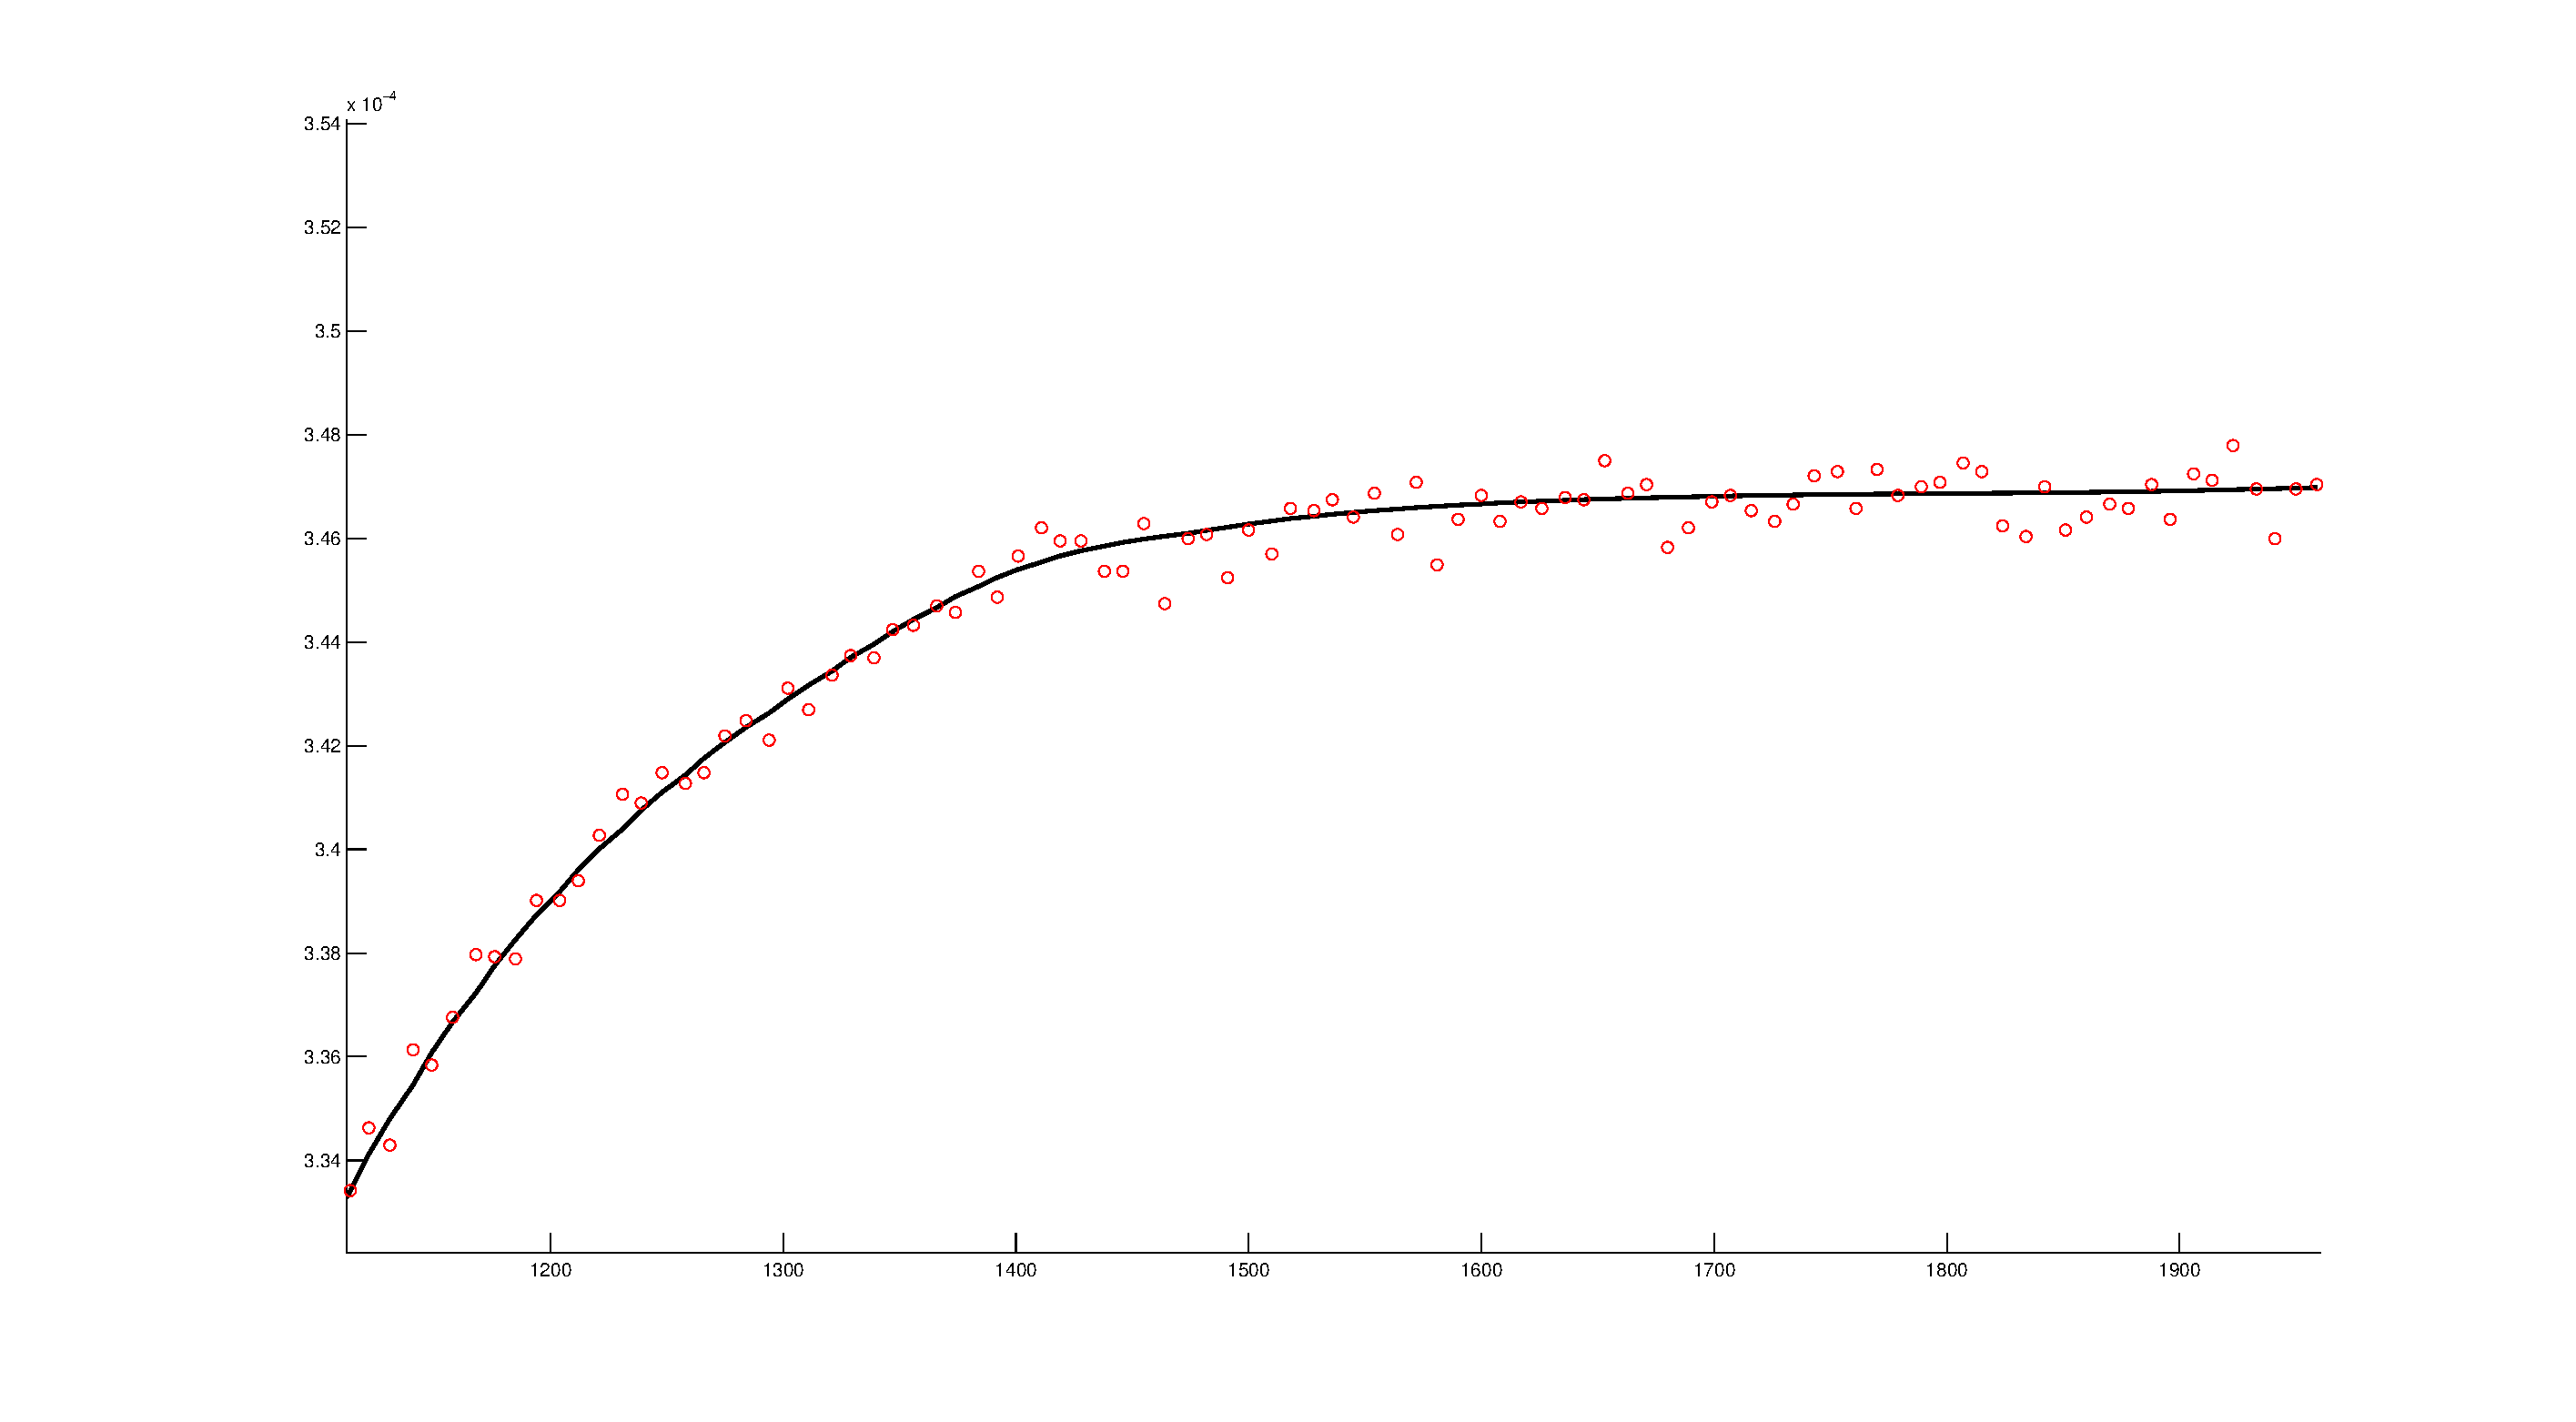
\includegraphics[scale=0.2]{loc_regr_b.eps}
\end{frame}

\begin{frame}
  \frametitle{Сплайны}
  \begin{itemize}
    \item Разбиваем $[a,b]$ на $k$ отрезков. На каждом отрезке строим оптимальный полином,
    учитывая краевые ограничения.
    \item Можем задавать дополнительные ограничения: выпуклость, монотонность, значение интеграла на отрезке, линейные участки.
    \item Можно аналитически посчитать производную.
  \end{itemize}
\end{frame}

\begin{frame}
  \frametitle{Сплайны}
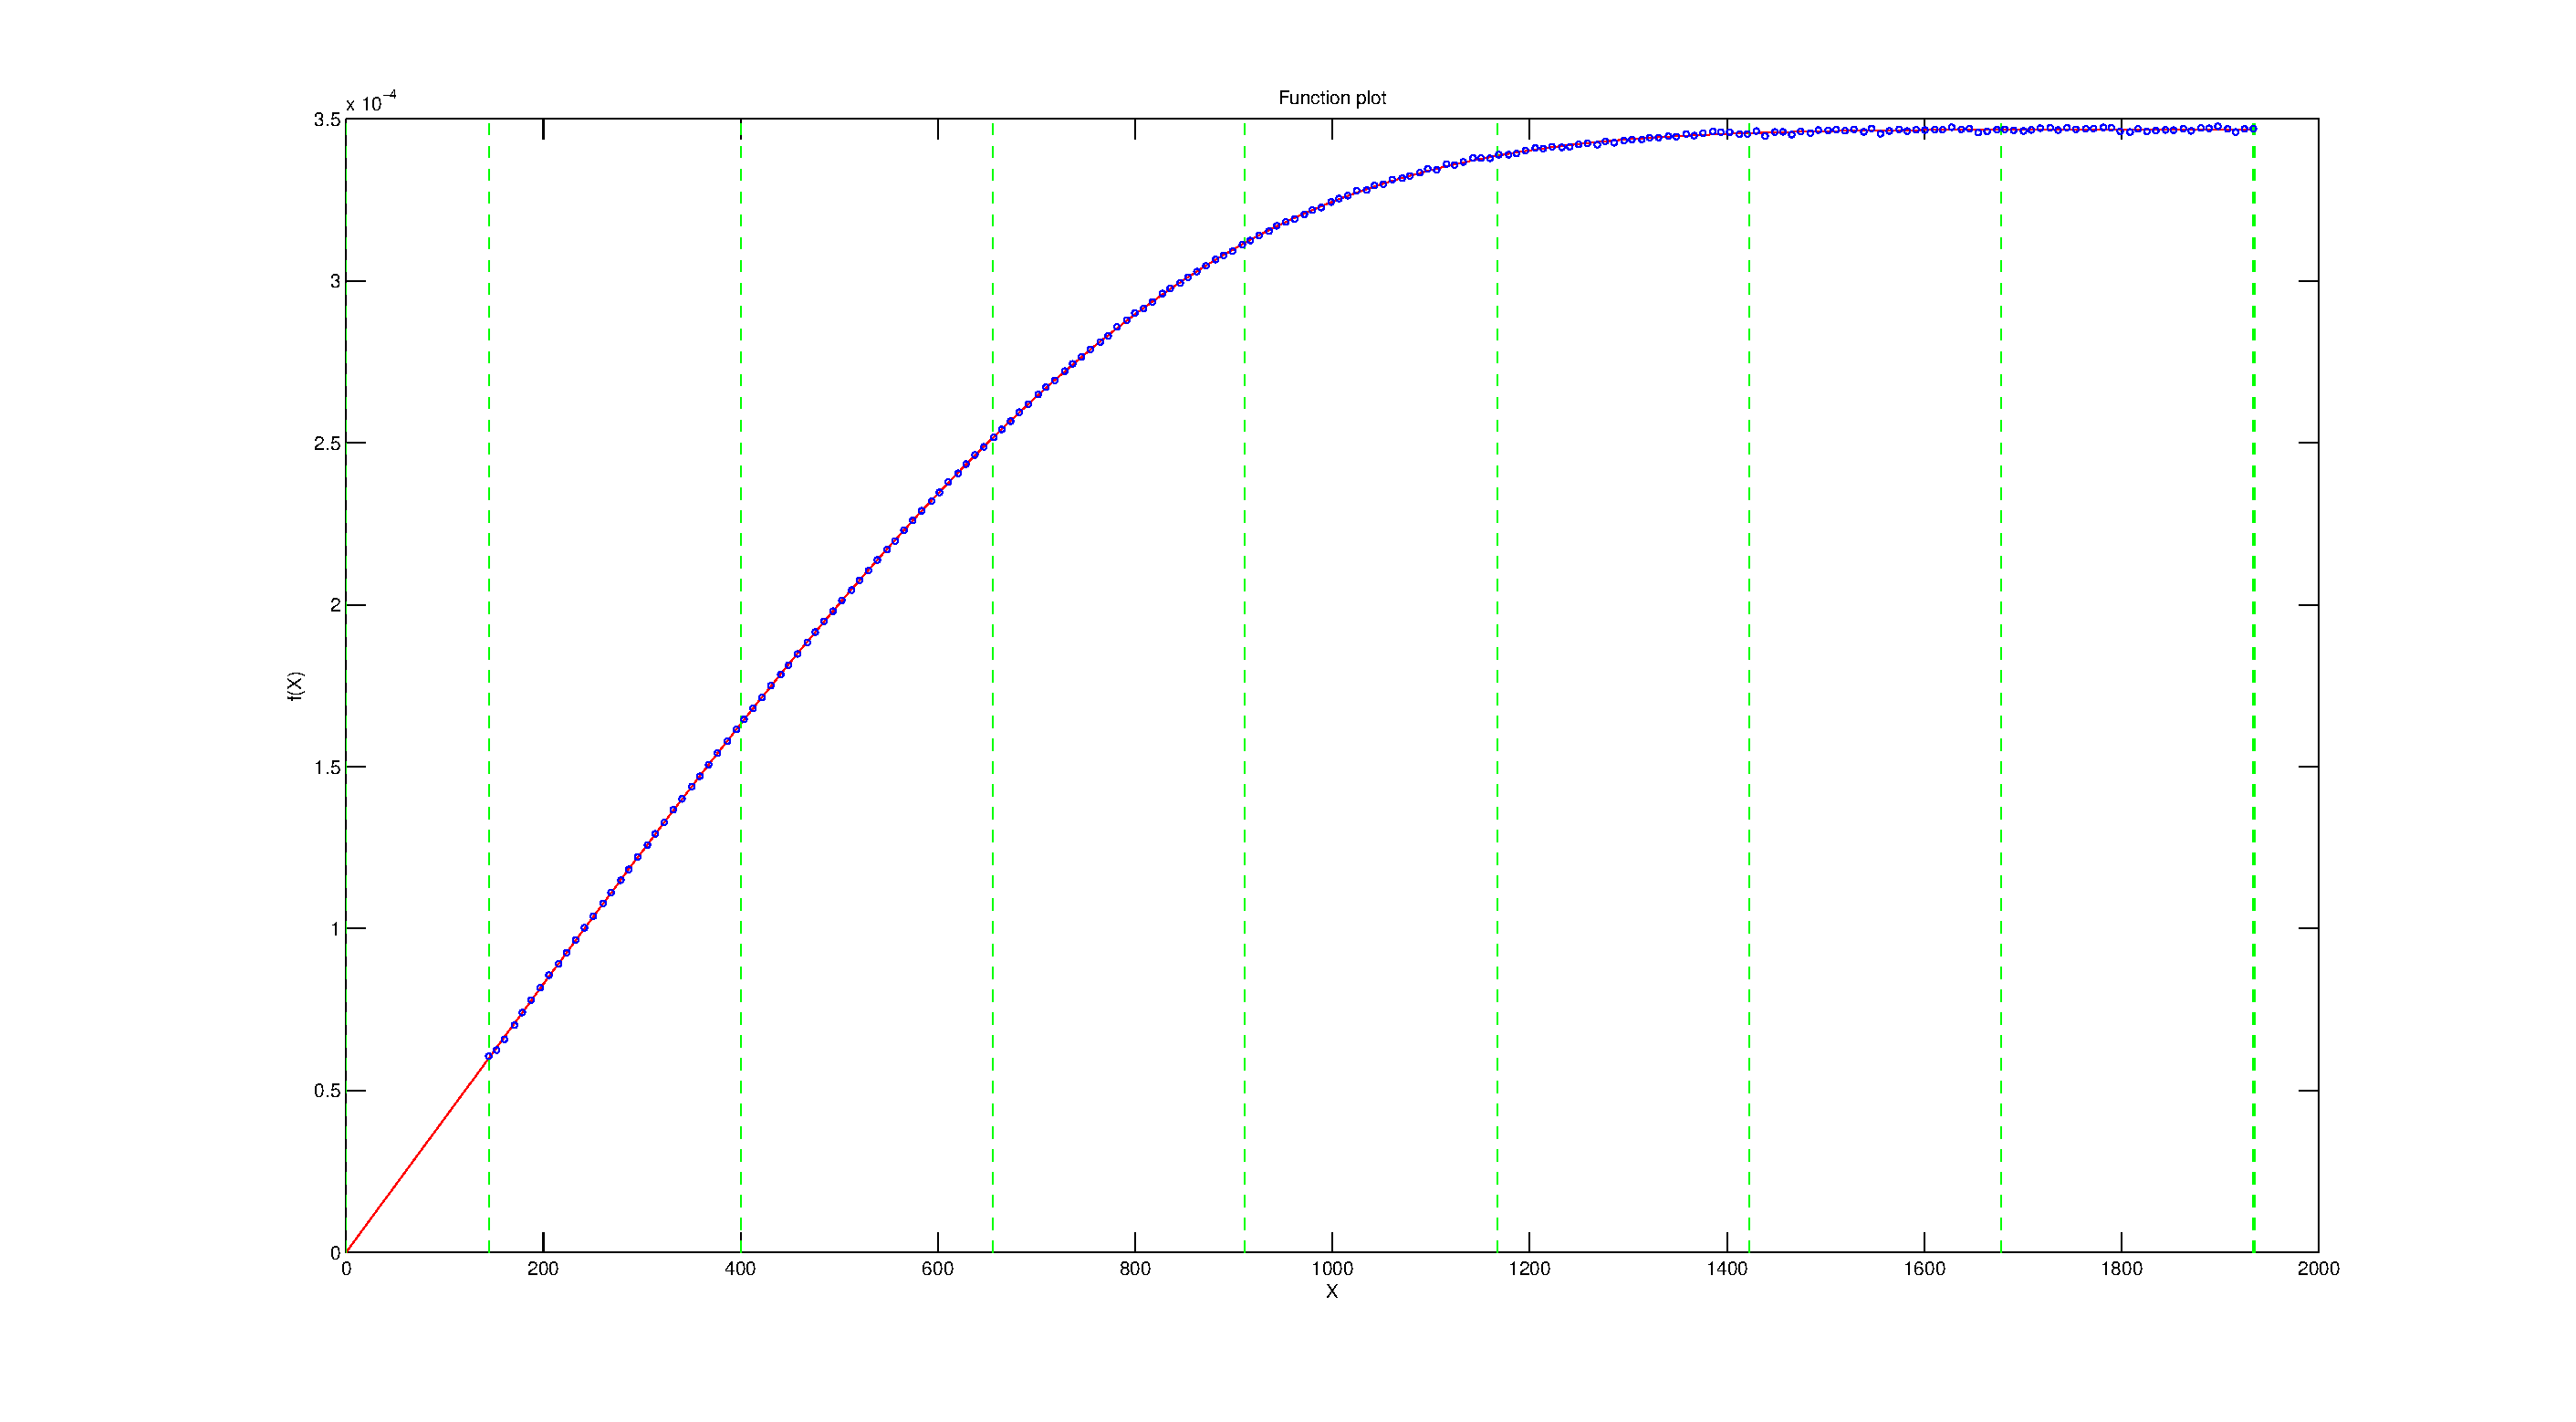
\includegraphics[scale=0.2]{spline.eps}
\end{frame}

\begin{frame}
  \frametitle{Сплайны}
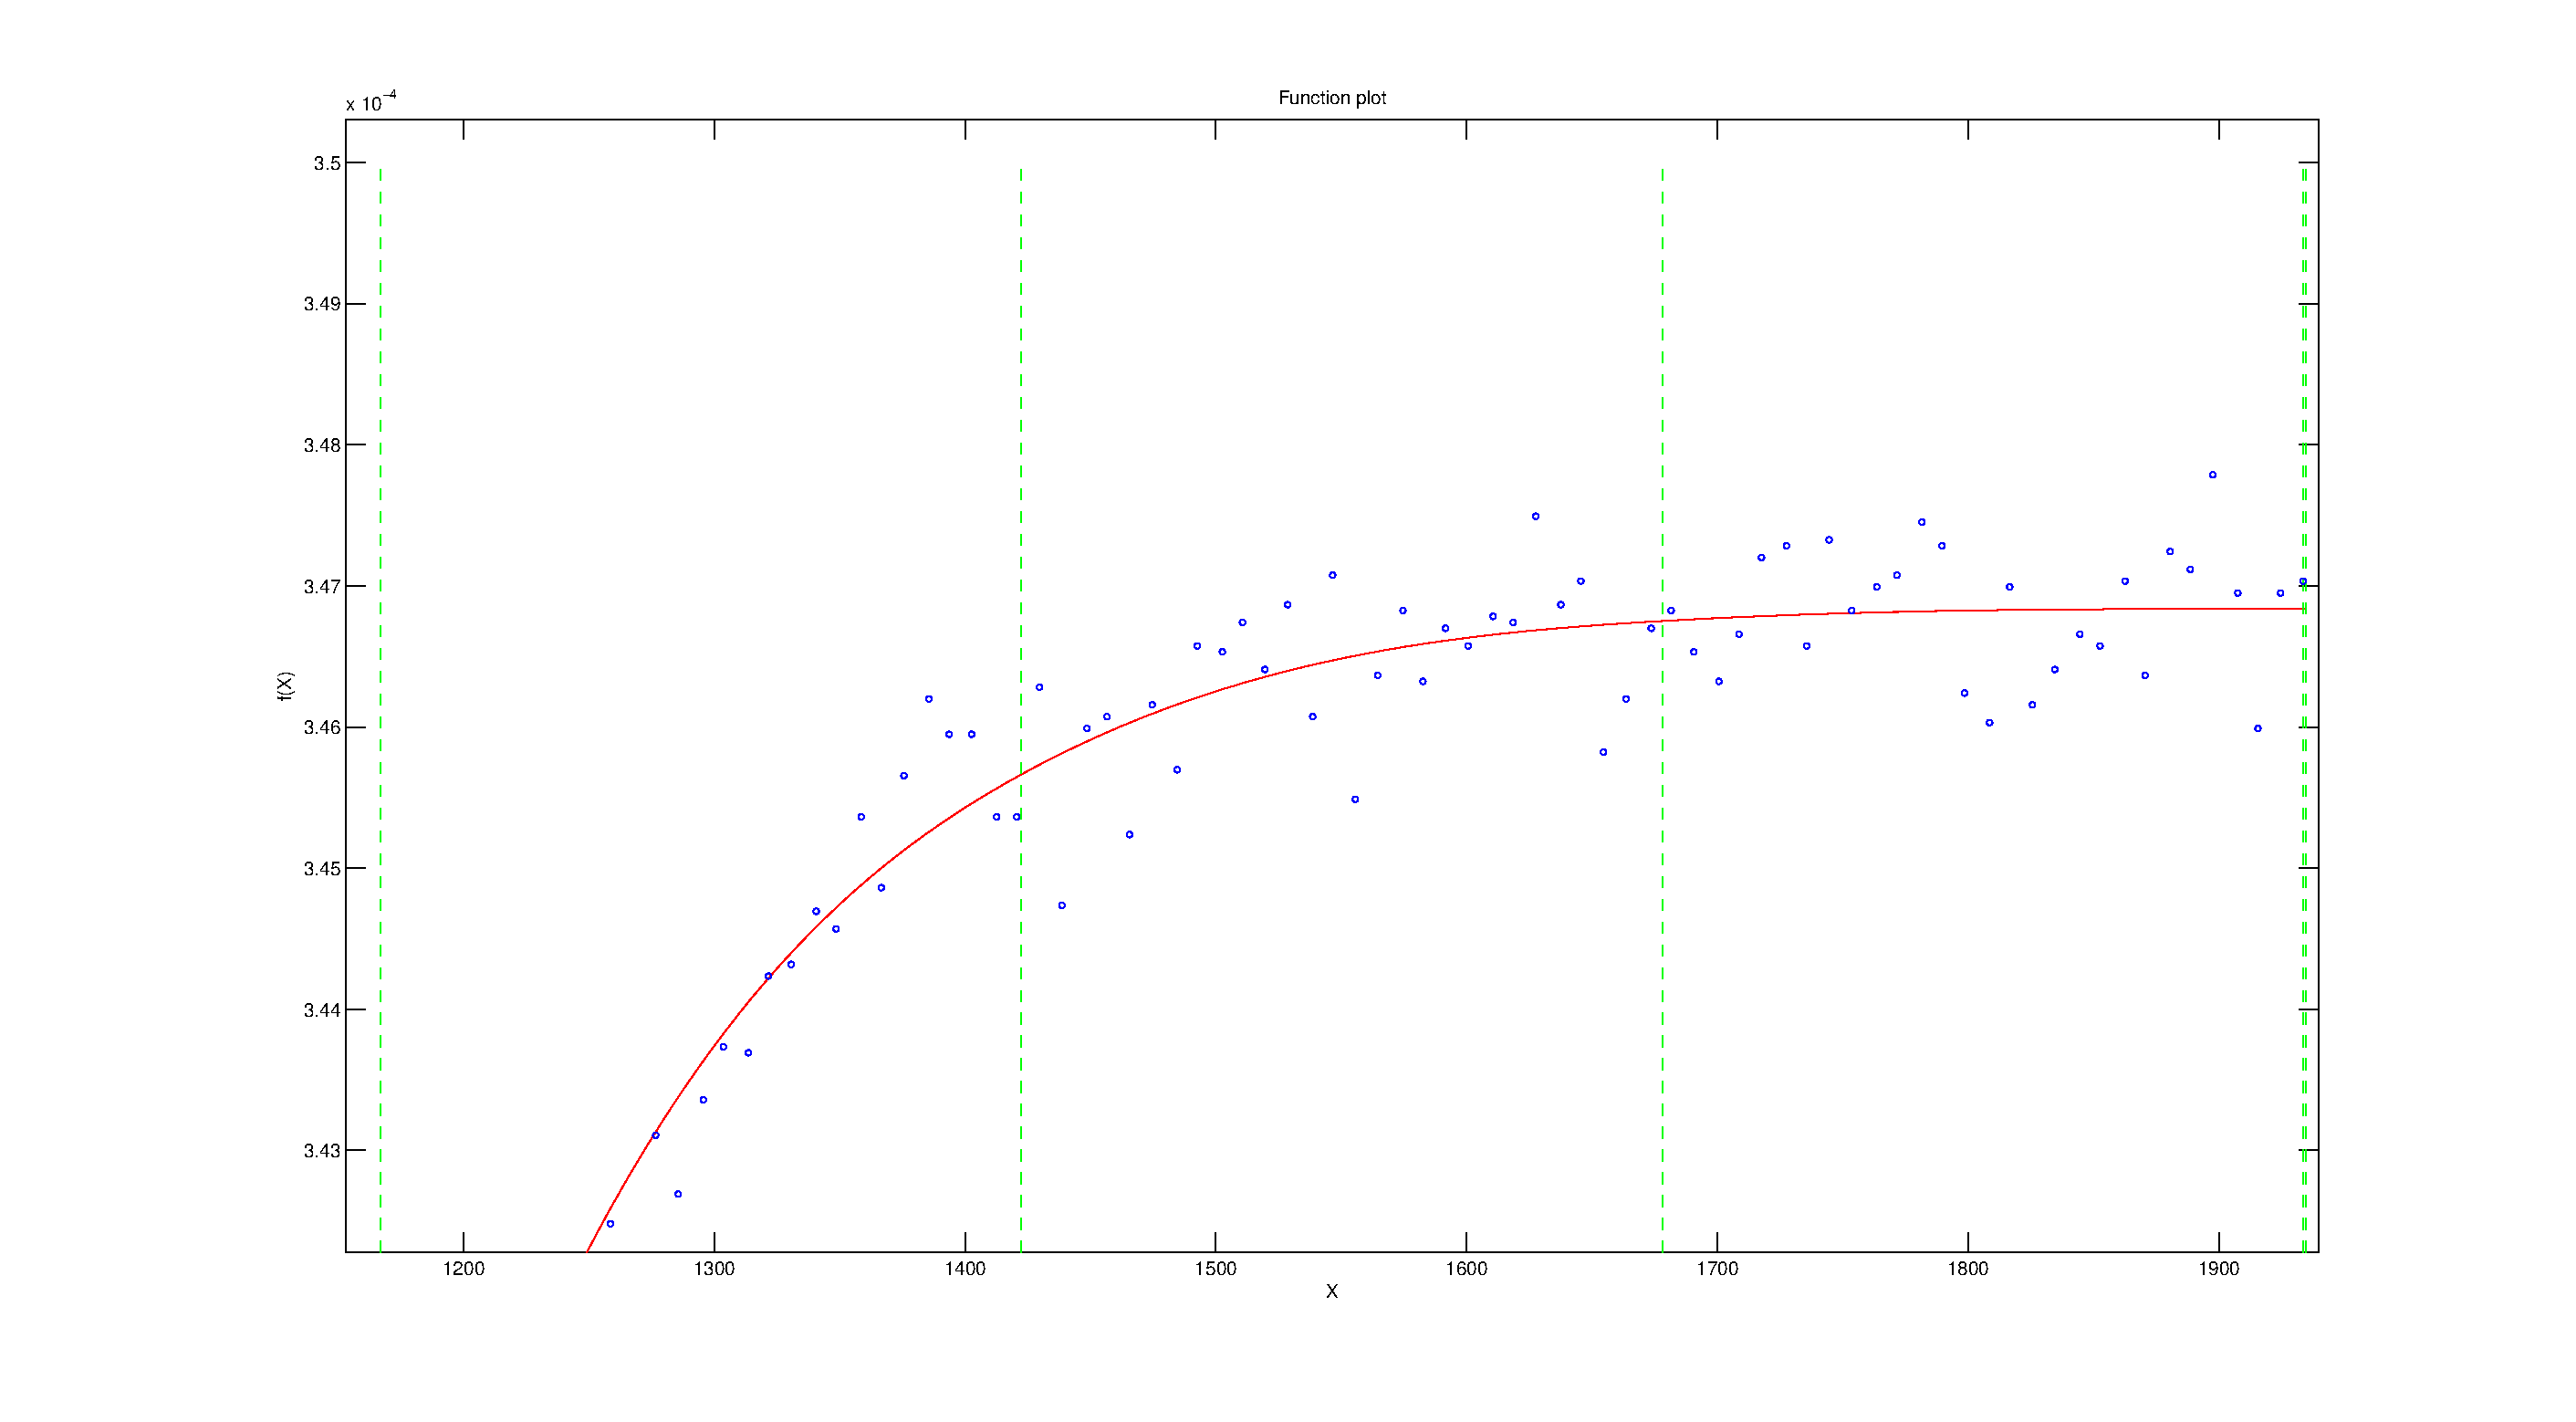
\includegraphics[scale=0.2]{spline_b.eps}
\end{frame}

\begin{frame}
  \frametitle{Smoothing(regression) splines}
  \begin{itemize}
    \item  $\displaystyle \sum_{i=1}^l \bigl(\hat{f}(x_i)-y_i\bigr)^2 + \lambda \int \! (\hat{f}''(t))^2 \, \mathrm{d}t \rightarrow min_{\hat{f}}$
    \item $\displaystyle \hat{f}(x) = \sum_{j=1}^lN_j(x)\theta_j$, где $N_j$~-- базис сплайна.
 \end{itemize}
\end{frame}

\begin{frame}
  \frametitle{Smoothing(regression) splines}
  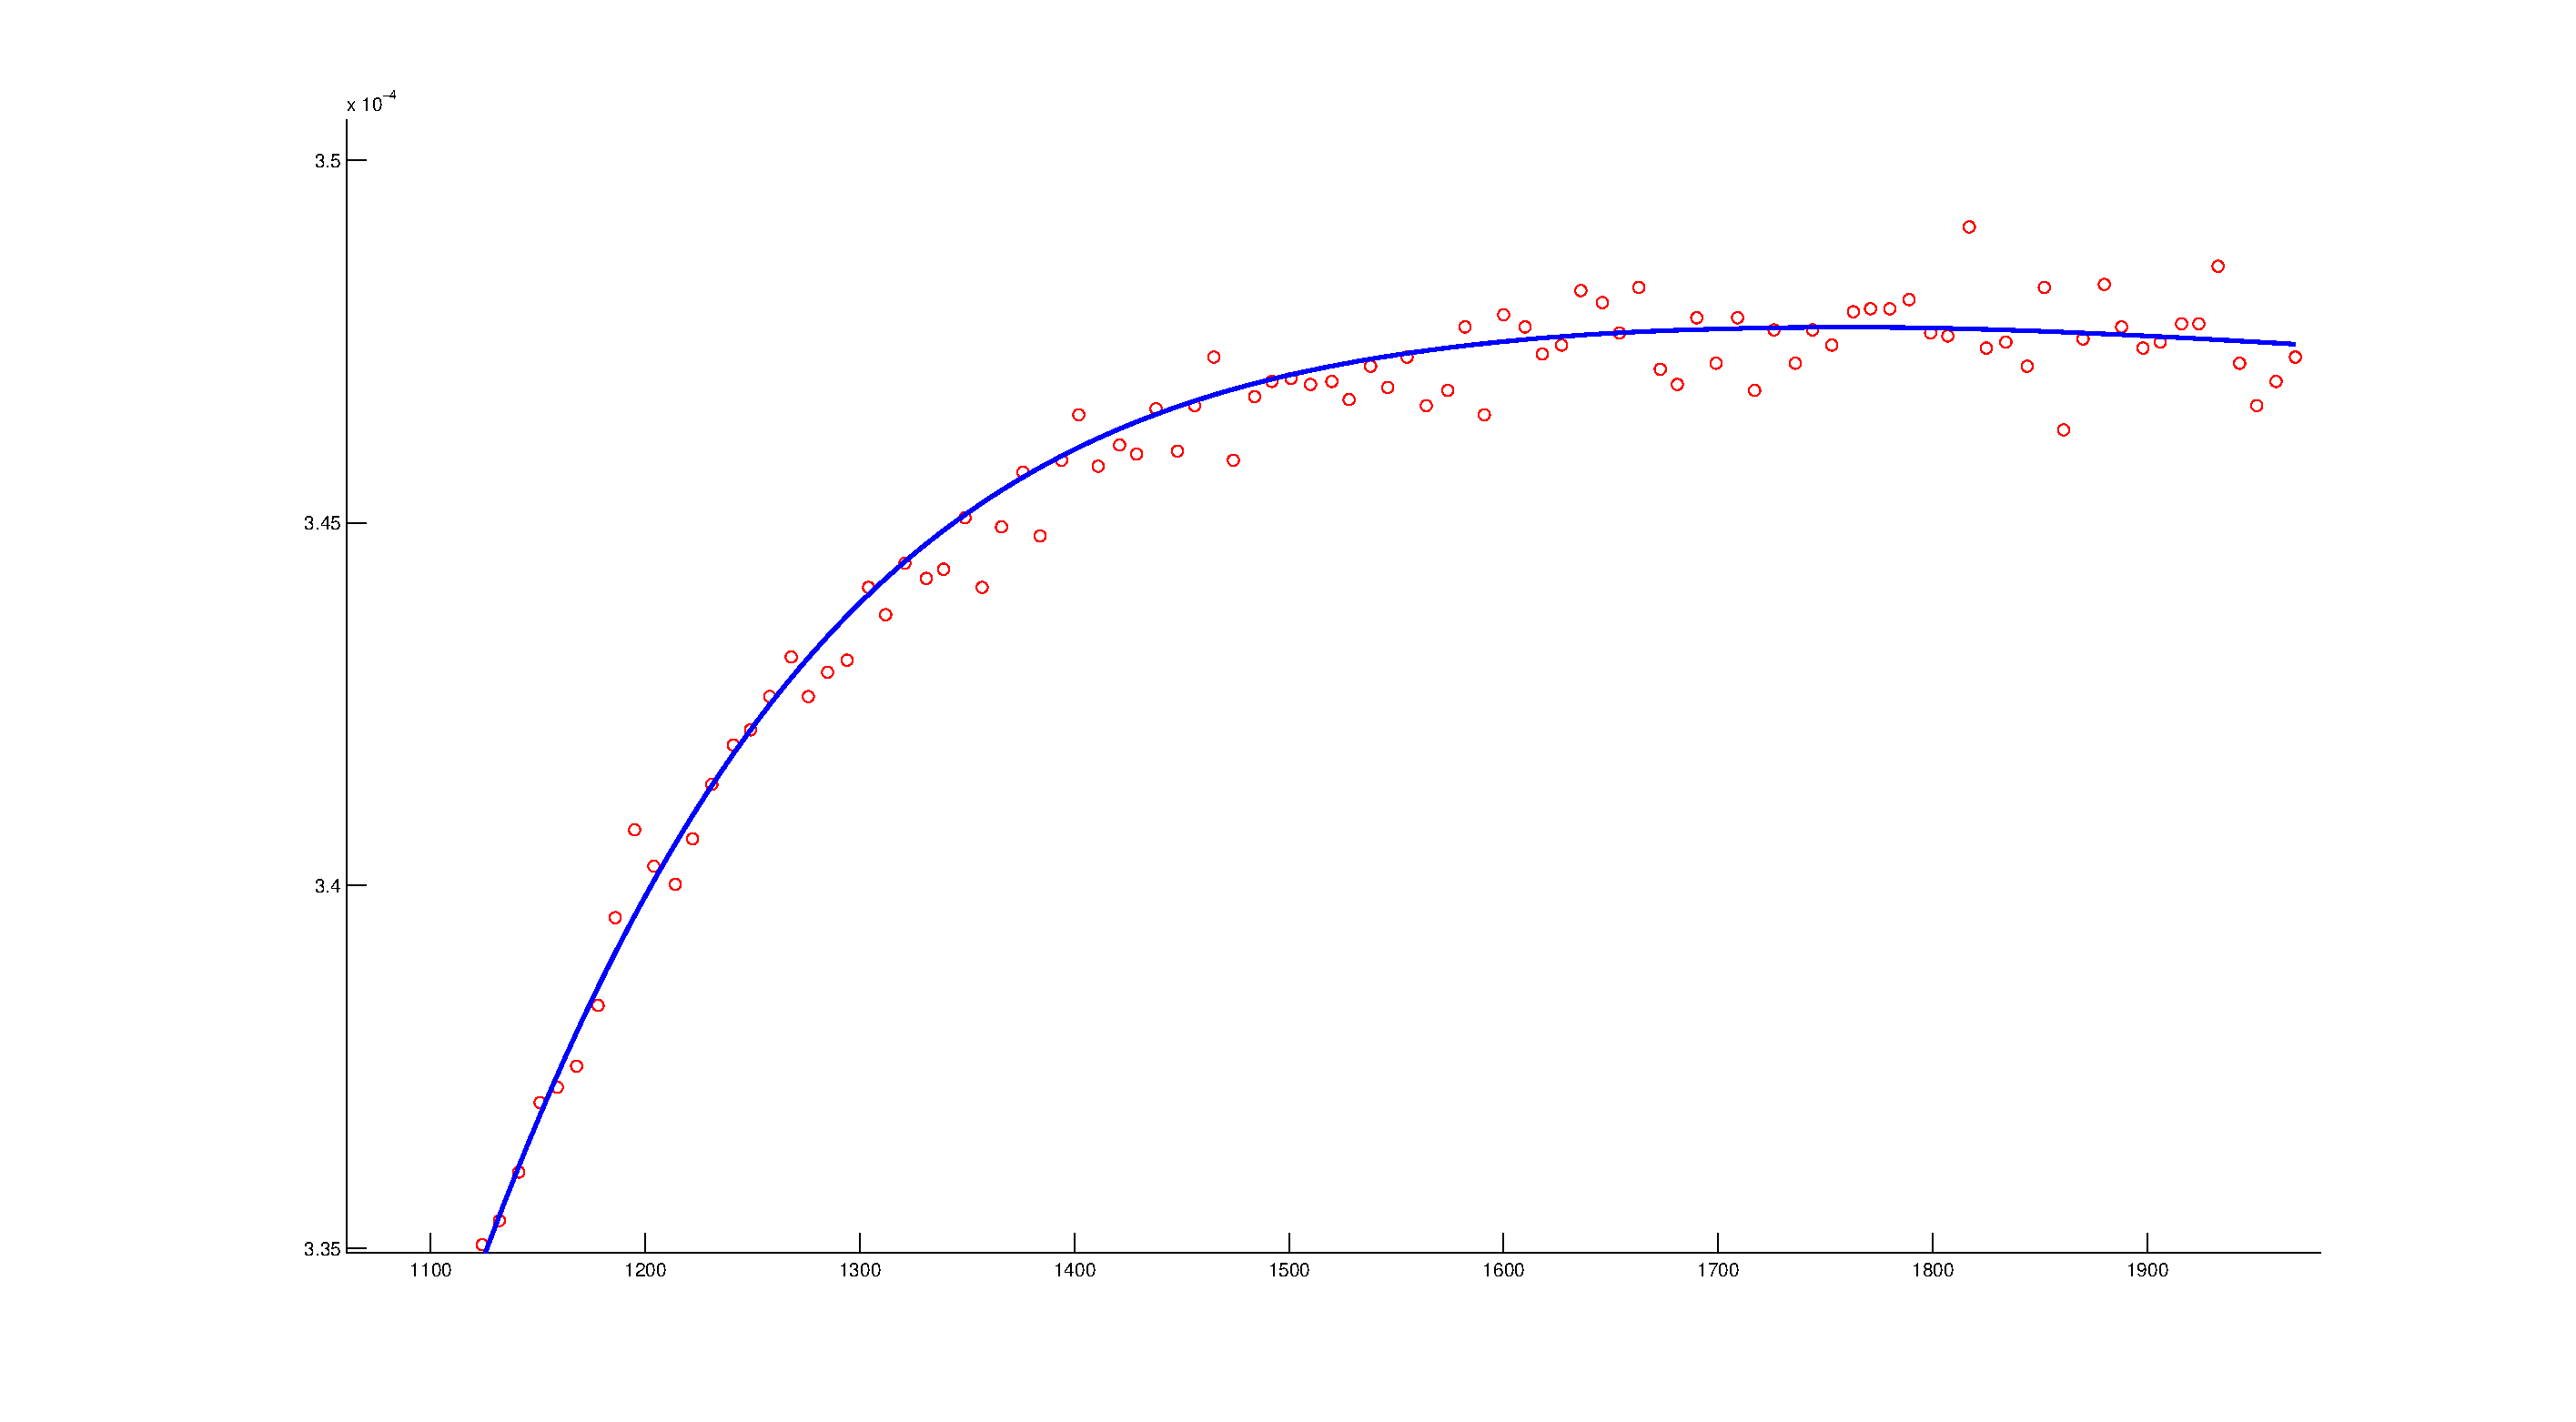
\includegraphics[scale=0.2]{smoothing_splines.eps}
\end{frame}

\subsection{Определение концентрации ферментов}
\begin{frame}
\frametitle{Определение концентрации ферментов}
\begin{itemize}
\item Рассматриваем реакцию одного субстрата. Известно, что в растворе могут присутствовать $N$ ферментов $e_1,...,e_N$.
\item Известны $k_{cat}^{(e_j,s)}$ и $K_M^{(e_j,s)}, j=1,\dots,N$. Требуется найти концентрации $E_j, j=1,\dots,N$  
\item $$
     & v=\frac{dP(t)}{dt}=\sum_{j=1}^N\frac{k_{cat}^{(e_j,s)}S(t)}{K_M^{(e_j,s)}+S(t)}E_j\\
 $$
\end{itemize}
\end{frame}


\begin{frame}
\frametitle{Материалы}
\begin{itemize}
\item Matlab, кусочное интерполирование сплайнами: SLM Tools, John D'Errico, 
http://www.mathworks.com/matlabcentral/fileexchange/24443-slm-shape-language-modeling
\item The Elements of Statistical Learning:Data Mining, Inference, and Prediction. Hastie T., Tibshirani R., Friedman J. 
http://www-stat.stanford.edu/\textasciitildetibs/ElemStatLearn/
\item Handbook of Computational Statistics. Gentle, James http://fedc.wiwi.hu-berlin.de/xplore/ebooks/html/csa/
\end{itemize}

\end{frame}

\end{document}

